%!TEX root = ../thesis.tex

\thispagestyle{myheadings}

\graphicspath{{Body/Figures/Wa/Datasets/Endgame/LostMuonFiles/MainCuts/}{Body/Figures/Wa/Datasets/ComparisonPlots/LostMuons/}{Body/Figures/Wa/Datasets/9d/SingleIteration/LostMuonFits/}{Body/Figures/Wa/Datasets/9d/PileupJobs/PileupGapTime/}{Body/Figures/Wa/Datasets/9d/PileupJobs/PileupDeadTime/auto-scaling/}{Body/Figures/Wa/Datasets/9d/PileupJobs/PileupDeadTime/fixed-scaling/}{Body/Figures/Wa/Datasets/9d/PileupJobs/PileupEnergyScale/}{Body/Figures/Wa/Datasets/9d/PileupJobs/PileupTimeShift/}{Body/Figures/Wa/Datasets/9d/SingleIteration/PileupMultiplierScan/}{Body/Figures/Wa/Datasets/60h/RatioConstruction/Ta/}{Body/Figures/Wa/Datasets/60h/RatioConstruction/TauMu/}{Body/Figures/Wa/Datasets/9d/Binning/BinEdge/}{Body/Figures/Wa/Datasets/9d/Binning/BinWidth/}{Body/Figures/Wa/Datasets/60h/Gain/0p25-steps/}{Body/Figures/Wa/Datasets/60h/Gain/Lifetime/}}




\section{Systematic errors}
\label{sec:SystematicErrors}


Evaluating the systematic errors which bias the \wa extraction is a major part of the precession frequency analysis. Systematic errors typically stem from sources which introduce time-dependent phases over the course of a fill,
    \begin{align} \label{eq:timeDependentPhase}
        \cos{(\omega_{a}t + \phi(t))} \rightarrow \cos{((\omega_{a}+\phi_{1})t + \phi_{0} + \phi_{2}t^{2} + ...)},
    \end{align}
where $\phi(t)$ can in general be expanded to higher orders. Because the phase is highly correlated to the extracted frequency, and because more decay positrons are detected at early times within a fill, a time-dependent phase pulls the extracted frequency away from it's real value. Sources of systematic uncertainty can be separated into several general categories. These include systematic errors in the pileup subtraction,  gain corrections, CBO fit model, muon losses, and E-field and pitch corrections, among others. In each case early-to-late shifts are a danger in the analysis and must be evaluated appropriately. \tabref{tab:wauncertainties} gives the target systematic uncertainties for the E989 experiment, which has the goal of a \SI{70}{ppb} systematic error on the precession frequency measurement. This represents a three to four-fold improvement over the E821 experiment systematic errors which were of order \SI{210}{} -- \SI{310}{ppb} depending on running period \cite{E821FinalReport}.

\begin{table}
\centering
\setlength\tabcolsep{10pt}
\renewcommand{\arraystretch}{1.2}
\begin{tabular*}{.8\linewidth}{@{\extracolsep{\fill}}lG}
  \hline
    \multicolumn{2}{c}{\textbf{Target \wa Systematic Uncertainties}} \\
  \hline\hline
    Sources of uncertainty & \multicolumn{1}{c}{E989 Goal (ppb)} \\
  \hline
    Pileup & 40 \\
    Gain changes & 20 \\
    CBO & 30 \\
    Lost muons & 20 \\
    E-field and pitch corrections & 30 \\
    Other & 30 \\
  \hline
    Quadrature sum & \sim70 \\
  \hline 
\end{tabular*}
\caption[Target systematic uncertainties in the precession frequency measurement]{Target systematic errors in the precession frequency measurement for the E989 experiment.}
\label{tab:wauncertainties}
\end{table}


Properly evaluated systematic errors should in general be static with respect to the amount of statistics. Run~1 of E989 consisted of more than four separate datasets with distinct running conditions, necessitating the need for independent systematic uncertainty evaluations. Such uncertainty evaluations for four of the Run~1 datasets are presented here. Systematic errors for the lost muon phase error and the the E-field and pitch corrections are dependent on analyses from other working groups. The numbers given here for them are preliminary estimations.



\subsection{Pileup systematic errors}
\label{sub:pileuperror}

As described in \secref{sub:pileupsubtraction}, the pileup background oscillates at \wa which by extension means a strong effect on the final fitted $R$ value. If the subtracted pileup spectrum is mis-constructed in any way, there will be a systematic error on $R$. In general the pileup systematic error can be separated into two parts, the error on the amplitude and the error on the phase. In order to estimate the two parts, the uncertainties on the pileup amplitude and phase need to be estimated along with the sensitivities of $R$ to them. \tabref{tab:histogramparameters} gives the default values used for the pileup construction parameters \{ADT, SDT, SGT, C\}. How these parameters feed into the amplitude and phase systematic errors will be discussed in turn, and the overall errors calculated for the different Run~1 datasets.


As a reminder the default values used for the ADT and SDT were \ns{5} each, and a default automatic pileup amplitude multiplier of $\sim1.03$ was applied to the pileup spectra. In order to calculate the systematic dependence on the choice of ADT or SDT, the SDT parameter was scanned over from \ns{5} to \ns{10} in steps of \ns{1}. This was done with and without the same automatic pileup amplitude scaling procedure as described in \secref{sub:pileupsubtraction}. The results of the study for the 9d dataset are shown in Figures~\ref{fig:SDTscan_noScaling} and \ref{fig:SDTscan_autoScaling}. In the case where there was no automatic scaling applied there is a clear minimum in the \chisq results and a steep slope in $R$ corresponding to a large sensitivity of $R$ to the choice of SDT. In the case where the automatic scaling was applied however, the minimum in the \chisq results has disappeared, while the sensitivity of $R$ has become much reduced to the point of no longer being a clear trend\footnote{This slope in $R$ varies between positive and negative values based on dataset, so there is no real clear trend in $R$.}. The fact that applying the automatic pileup amplitude scaling produces nearly identical pileup spectra with no clear trend in $R$ regardless of the choice of SDT (and by extension ADT), any systematic error due to the choice of these two parameters can be subsumed into the direct pileup amplitude error itself, discussed down below. It should be noted in fact that the choices of ADT and SDT are largely irrelevant barring statistics, as the automatic amplitude scaling procedure can always account for any differences between the two. 


\begin{figure}
\centering
    \begin{subfigure}[t]{0.45\textwidth}
        \centering
        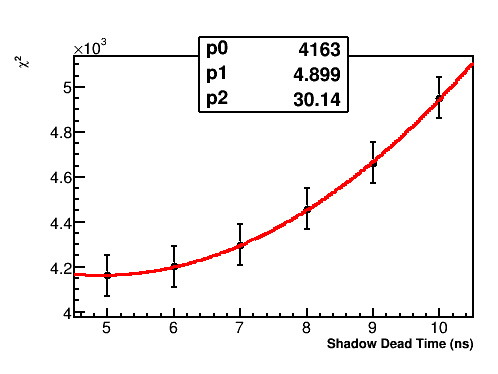
\includegraphics[width=\textwidth]{FullRatio_Chi2_Vs_ShadowDeadTime_Canv_9d_fixed}
        \caption{\chisq versus SDT. The parabolic fit equation used was $y = p_{2}(x - p_{1})^{2} + p_{0}.$}
    \end{subfigure}% %you need this % here to add spacing between subfigures
    \hspace{1cm}
    \begin{subfigure}[t]{0.45\textwidth}
        \centering
        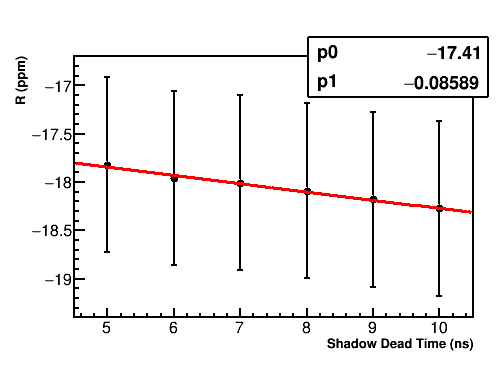
\includegraphics[width=\textwidth]{FullRatio_R_Vs_ShadowDeadTime_Canv_9d_fixed}
        \caption{$R$ versus SDT. The parameter $p_{1}$ gives the sensitivity of $R$ to the value of SDT, with units in ppm/ns.}
    \end{subfigure}

    \begin{subfigure}[t]{0.45\textwidth}
        \centering
        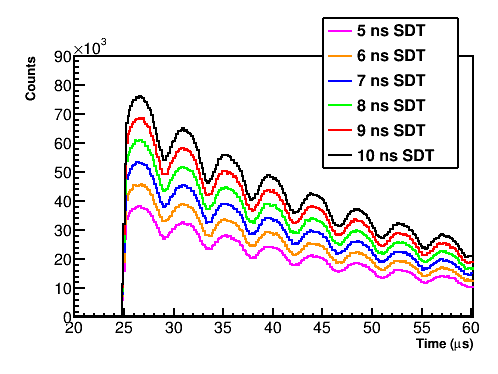
\includegraphics[width=\textwidth]{SDT_PileupTimeComparison_9d_fixed}
        \caption{The pileup time spectrum for different choices of SDT.}
    \end{subfigure}% %you need this % here to add spacing between subfigures
    \hspace{1cm}
    \begin{subfigure}[t]{0.45\textwidth}
        \centering
        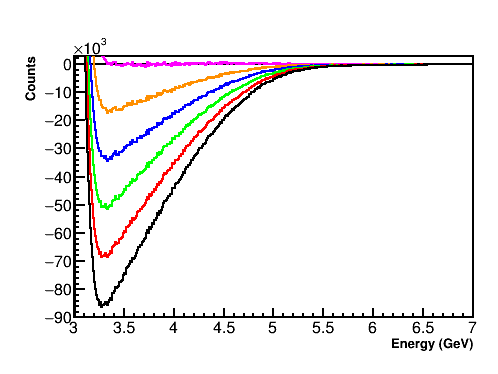
\includegraphics[width=\textwidth]{SDT_CorrEnergyComparison_9d_fixed}
        \caption{The corrected energy spectrum for different choices of SDT.}
    \end{subfigure}
\caption[Pileup shadow dead time scan without automatic pileup amplitude scaling]{Shadow dead time scan results without automatic pileup amplitude scaling. A clear minimum in the \chisq plot is seen near \ns{5} corresponding to the choice of ADT, and a large sensitivity for $R$ is observed. In the bottom two spectra plots the magenta curve corresponds to a choice SDT = \ns{5} while the black curve corresponds to SDT = \ns{10}. The larger choice of SDT leads to a greater estimation of the pileup, which as shown in the energy spectra plot leads to a corresponding over-subtraction at energies where hits consist mostly or purely of pileup pulses. Data are from the 9d dataset.}
\label{fig:SDTscan_noScaling}
\end{figure}


\begin{figure}
\centering
    \begin{subfigure}[t]{0.45\textwidth}
        \centering
        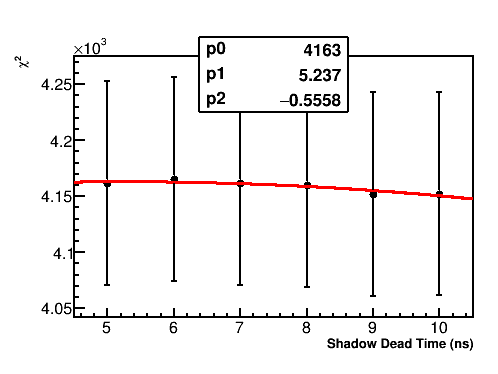
\includegraphics[width=\textwidth]{FullRatio_Chi2_Vs_ShadowDeadTime_Canv_9d_auto}
        \caption{\chisq versus SDT. The parabolic fit equation used was $y = p_{2}(x - p_{1})^{2} + p_{0}.$}
    \end{subfigure}% %you need this % here to add spacing between subfigures
    \hspace{1cm}
    \begin{subfigure}[t]{0.45\textwidth}
        \centering
        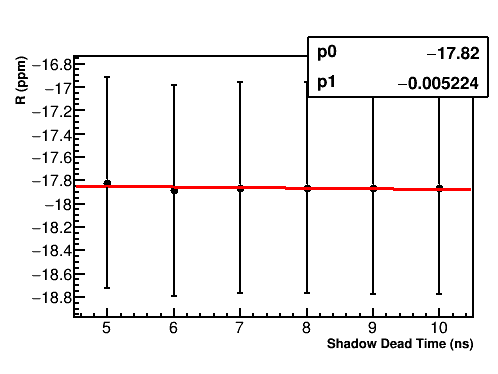
\includegraphics[width=\textwidth]{FullRatio_R_Vs_ShadowDeadTime_Canv_9d_auto}
        \caption{$R$ versus SDT. The parameter $p_{1}$ gives the sensitivity of $R$ to the value of SDT, with units in ppm/ns.}
    \end{subfigure}

    \begin{subfigure}[t]{0.45\textwidth}
        \centering
        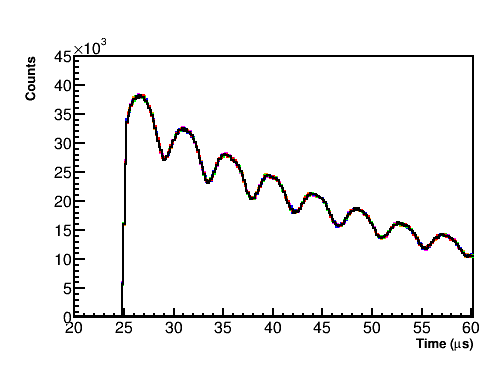
\includegraphics[width=\textwidth]{SDT_PileupTimeComparison_9d_auto}
        \caption{The pileup time spectrum for different choices of SDT.}
    \end{subfigure}% %you need this % here to add spacing between subfigures
    \hspace{1cm}
    \begin{subfigure}[t]{0.45\textwidth}
        \centering
        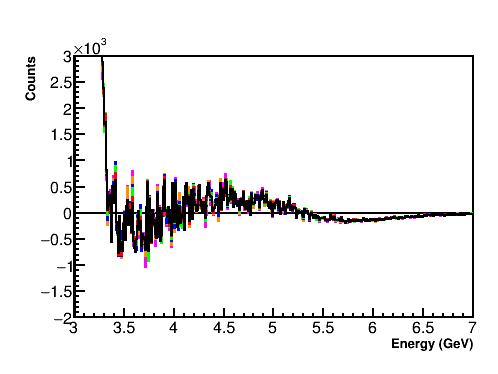
\includegraphics[width=\textwidth]{SDT_CorrEnergyComparison_9d_auto}
        \caption{The corrected energy spectrum for different choices of SDT.}
    \end{subfigure}
\caption[Pileup shadow dead time scan with automatic pileup amplitude scaling]{Shadow dead time scan results with automatic pileup amplitude scaling. No clear minimum is observed in the \chisq plot, and the sensitivity for $R$ is small. In the bottom two spectra plots the magenta curve corresponds to a choice SDT = \ns{5} while the black curve corresponds to SDT = \ns{10}. With the automatic amplitude scaling applied, the time and energy spectra are nearly identical and lie on top of each other. That combined with the lack of clear minimum in the \chisq plot and no clear sensitivity in $R$ indicate that there is no real systematic error due to the choice of SDT. Data are from the 9d dataset.}
\label{fig:SDTscan_autoScaling}
\end{figure}


In order to calculate the systematic dependence on the choice of SGT (default value of \ns{10}), the SGT parameter was scanned over from \ns{10} to \ns{20} in steps of \ns{1}. The results of the study with the automatic pileup amplitude scaling applied is shown in \figref{fig:SGTscan}. Just as in the SDT scan with the automatic pileup amplitude scaling, there is no minimum in the \chisq results, the sensitivity of $R$ to the value of SGT not so clear, and the pileup spectra for the various choices of SGT are nearly identical. Therefore again any systematic error due to the choice of SGT is subsumed into the pileup amplitude error.


\begin{figure}
\centering
    \begin{subfigure}[t]{0.45\textwidth}
        \centering
        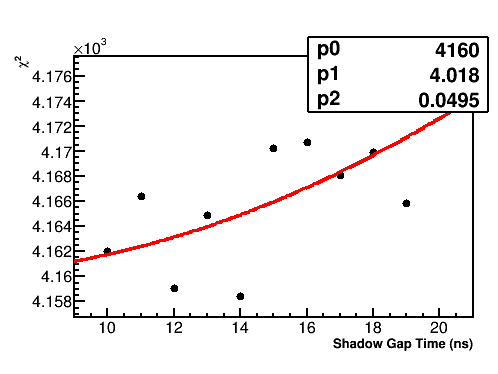
\includegraphics[width=\textwidth]{FullRatio_Chi2_Vs_ShadowGapTime_Canv_9d}
        \caption{\chisq versus SGT. The parabolic fit equation used was $y = p_{2}(x - p_{1})^{2} + p_{0}.$}
    \end{subfigure}% %you need this % here to add spacing between subfigures
    \hspace{1cm}
    \begin{subfigure}[t]{0.45\textwidth}
        \centering
        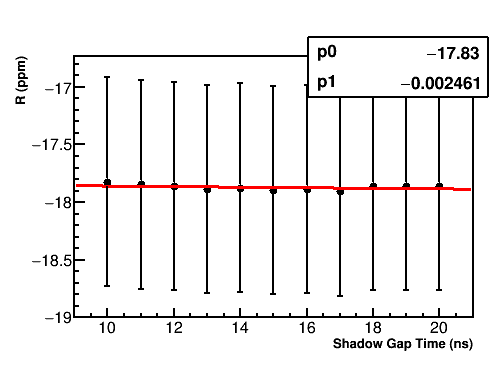
\includegraphics[width=\textwidth]{FullRatio_R_Vs_ShadowGapTime_Canv_9d}
        \caption{$R$ versus SGT. The parameter $p_{1}$ gives the sensitivity of $R$ to the value of SGT, with units in ppm/ns.}
    \end{subfigure}

    \begin{subfigure}[t]{0.45\textwidth}
        \centering
        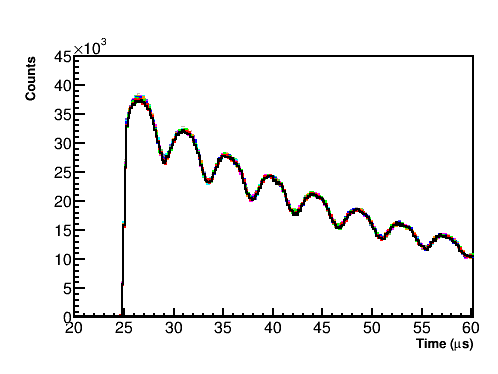
\includegraphics[width=\textwidth]{SGT_PileupTimeComparison_9d}
        \caption{The pileup time spectrum for different choices of SGT.}
    \end{subfigure}% %you need this % here to add spacing between subfigures
    \hspace{1cm}
    \begin{subfigure}[t]{0.45\textwidth}
        \centering
        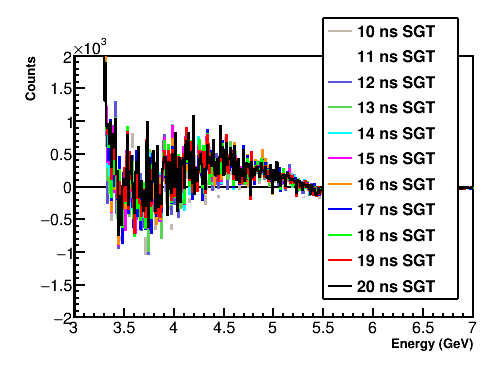
\includegraphics[width=\textwidth]{SGT_CorrEnergyComparison_9d}
        \caption{The corrected energy spectrum for different choices of SGT.}
    \end{subfigure}
\caption[Pileup shadow gap time scan with automatic pileup amplitude scaling]{Shadow gap time scan results with automatic pileup amplitude scaling. No clear minimum is observed in the \chisq plot, and the trend for $R$ isn't clear, with points fluctuating above and below the fit curve. In the bottom two spectra plots one of the gray curves (hidden) corresponds to a choice SGT = \ns{10} while the black curve corresponds to SGT = \ns{20}. With the automatic amplitude scaling applied, the time and energy spectra lie on top of each other. That combined with the lack of clear minimum in the \chisq plot and small sensitivity in $R$ indicate that there is no real systematic error due to the choice of SGT. Data are from the 9d dataset.}
\label{fig:SGTscan}
\end{figure}


The pileup amplitude systematic error is the error on $R$ assuming the scale of the pileup was incorrectly constructed. In order to evaluate this error, multipliers were applied to the pileup spectra from 0.9 to 1.1 in steps of 0.01 (dropping the default automatic pileup scaling of $\sim1.03$ mentioned before). The data was then re-fit to find the change in $R$. The results of the study for the 9d dataset are shown in \figref{fig:PMscan}. As shown there is a clear minimum near 1 in the \chisq results and a large sensitivity of $R$ to the multiplier. The systematic error on $R$ is calculated as 
    \begin{align}
        \delta R = \sigma_{P_{m}} \times \frac{dR}{dP_{m}},
    \end{align}
where $P_{m}$ is the value of the pileup multiplier. The error $\sigma_{P_{m}}$ is calculated as the width of the fitted parabola in the \chisq plot, defined as the change in $P_{m}$ from the minimum for the \chisq to increase by 1. This is calculated as 
    \begin{align}
        \sigma_{P_{m}} = \sqrt{\frac{2}{f''(\chi^{2})}} = \frac{1}{\sqrt{p_{2}}},
    \end{align}
where $p_{2}$ is the fit parameter as given in the top right of the \chisq plot. The sensitivities of $R$ to the pileup multiplier, uncertainties in the pileup amplitude, and final corresponding systematic errors for the Run~1 precession frequency analysis datasets are given in \tabref{tab:systematicError_pileupMultplier}. As shown in the table, the uncertainties on the pileup amplitude are of order 2 to 5\%, while the systematic errors on $R$ are on the order of \SI{10}{} to \SI{20}{ppb} depending on dataset.  It should be noted that the default automatic pileup multiplier of $\sim1.03$ does not necessarily correspond to the minimum in the \chisq plot, but is within $1\sigma$ of 1 or the minimum (except the Endgame which is closer to $2\sigma$)\footnote{Monte-Carlo tests with various random seeds showed this minimum fluctuating above and below 1. The distance from 1 therefore is not a good measure for the uncertainty in the pileup amplitude compared to the width of the \chisq parabola fit.}.


\begin{figure}
\centering
    \begin{subfigure}[t]{0.45\textwidth}
        \centering
        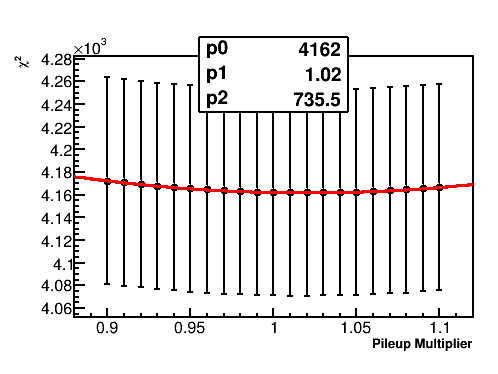
\includegraphics[width=\textwidth]{FullRatio_Chi2_Vs_PileupMultiplier_Canv_9d}
        \caption{\chisq versus pileup multiplier. The parabolic fit equation used was $y = p_{2}(x - p_{1})^{2} + p_{0}.$}
    \end{subfigure}% %you need this % here to add spacing between subfigures
    \hspace{1cm}
    \begin{subfigure}[t]{0.45\textwidth}
        \centering
        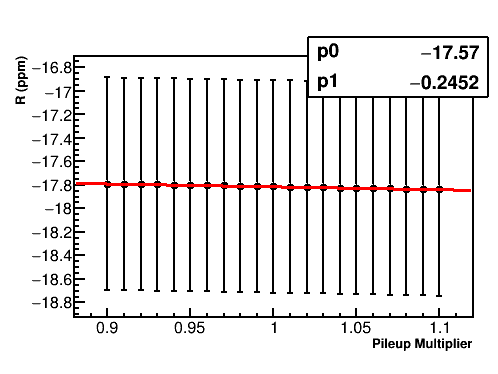
\includegraphics[width=\textwidth]{FullRatio_R_Vs_PileupMultiplier_Canv_9d}
        \caption{$R$ versus pileup multiplier. The parameter $p_{1}$ gives the sensitivity of $R$ to the value of the pileup multiplier, with units in ppm.}
    \end{subfigure}
\caption[Pileup multiplier scan]{Pileup multiplier scan. Data are from the 9d dataset.}
\label{fig:PMscan}
\end{figure}


\begin{table}
\centering
% \small
\setlength\tabcolsep{10pt}
\renewcommand{\arraystretch}{1.2}
\begin{tabular*}{0.65\linewidth}{@{\extracolsep{\fill}}lcccK}
% \begin{tabular}{@{\extracolsep{\fill}}lcccK}
  \hline
    \multicolumn{5}{c}{\textbf{Systematic Error due to Pileup Amplitude}} \\
  \hline\hline
    Dataset & \multicolumn{1}{c}{$dR/dP_{m}$} & $\sigma_{P_{m}}$ & $P_{m_{\text{min}}}$ & \multicolumn{1}{c}{$\boldsymbol{\delta R}$} \\
  \hline
    60h & $-419.3$ & 0.053 & 0.993 & 22.2 \\
    HighKick & $-372.8$ & 0.051 & 0.997 & 19.0 \\
    9d & $-245.2$ & 0.037 & 1.020 & 9.0 \\ 
    Endgame & $-335.3$ & 0.028 & 0.985 & 9.4 \\
  \hline
\end{tabular*}
\caption[Systematic error due to pileup amplitude]{Systematic error due to the pileup amplitude in the Ratio Method fits for the Run~1 precession frequency analysis datasets. The bold column gives the systematic error on \R. Units for $dR/dP_{m}$ and $\delta R$ are in ppb.}
\label{tab:systematicError_pileupMultplier}
\end{table}


The pileup phase error is the error on $R$ assuming the phase of the pileup was incorrectly constructed. This is separated into two parts. The first part is calculated by applying time-shifts to $t_{\text{doublet}}$ as given in \equref{eq:tdoublet}. Doing this artificially applies a phase shift to the pileup time spectrum. The data is then re-fit with the different pileup spectra and the change in $R$ is calculated. \figref{fig:PTSscan} shows the study results for the 9d dataset with time-shifts applied between \ns{-10} and \ns{10} in steps of \ns{1}. A clear sensitivity of $R$ to the value of time-shift is observed, however there is no clear minimum in the \chisq results. Because the width of the \chisq parabolic fit cannot be taken as the uncertainty in the pileup time-shift parameter , instead the uncertainty is taken conservatively at half the ADT at \ns{2.5}. The systematic error is calculated in the same way as for the pileup amplitude uncertainty,
    \begin{align}
        \delta R = \sigma_{P_{t}} \times \frac{dR}{dP_{t}},
    \end{align}
where $P_{t}$ is the value of the pileup time-shift. The sensitivities of $R$ to the pileup time-shift and corresponding systematic errors for the Run~1 precession frequency analysis datasets are given in \tabref{tab:systematicError_pileupTimeShift}.


\begin{figure}
\centering
    \begin{subfigure}[t]{0.45\textwidth}
        \centering
        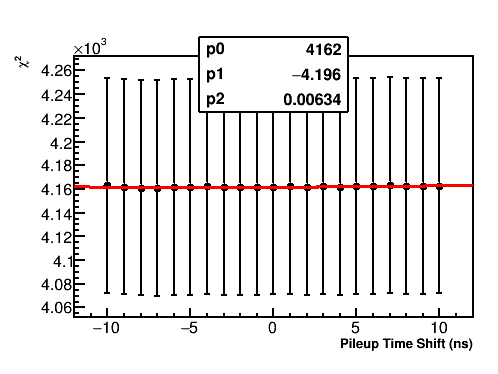
\includegraphics[width=\textwidth]{FullRatio_Chi2_Vs_PileupTimeShift_Canv_9d}
        \caption{\chisq versus pileup time-shift. There is no clear minimum in the plot.} 
    \end{subfigure}% %you need this % here to add spacing between subfigures
    \hspace{1cm}
    \begin{subfigure}[t]{0.45\textwidth}
        \centering
        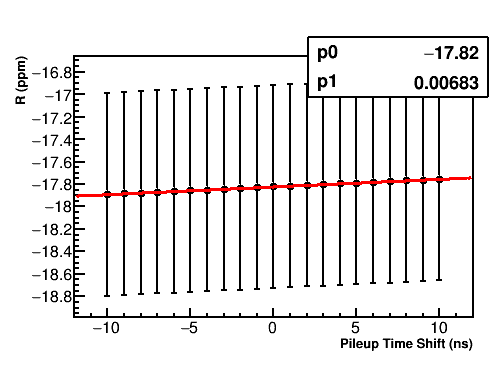
\includegraphics[width=\textwidth]{FullRatio_R_Vs_PileupTimeShift_Canv_9d}
        \caption{$R$ versus pileup time-shift. The parameter $p_{1}$ gives the sensitivity of $R$ to the value of the pile time-shift, with units in ppm/ns.}
    \end{subfigure}
\caption[Pileup time-shift scan]{Scan over pileup time-shift. Data are from the 9d dataset.}
\label{fig:PTSscan}
\end{figure}


\begin{table}
\centering
% \small
\setlength\tabcolsep{20pt}
\renewcommand{\arraystretch}{1.2}
\begin{tabular*}{0.7\linewidth}{@{\extracolsep{\fill}}lccK}
% \begin{tabular}{@{\extracolsep{\fill}}lcccK}
  \hline
    \multicolumn{4}{c}{\textbf{Systematic Error due to Pileup Time Shift}} \\
  \hline\hline
    Dataset & & \multicolumn{1}{c}{$dR/dP_{t}$} & \multicolumn{1}{c}{$\boldsymbol{\delta R}$} \\
  \hline
    60h & & 7.0 & 17.6 \\
    HighKick & & 7.6 & 19.0 \\
    9d & & 6.8 & 17.1 \\ 
    Endgame & & 5.7 & 14.3 \\
  \hline
\end{tabular*}
\caption[Systematic error due to pileup time shift]{Systematic error due to the pileup time-shift parameter $P_{t}$ in the Ratio Method fits for the Run~1 precession frequency analysis datasets. The bold column gives the systematic error on \R. Units for $dR/dP_{t}$ and $\delta R$ are in ppb/ns and ppb respectively. The error on the $P_{t}$ is by default taken to be \ns{2.5} as described in the text.}
\label{tab:systematicError_pileupTimeShift}
\end{table}


% -maybe put in fit start time scan of various time shifts converging to one
% -maybe add plot of nice energy threshold where pileup goes smooth and phase error would disappear


The second part of the pileup phase error comes from the choice of constant $C$ in the calculation of $E_{\text{doublet}}$ as given in \equref{eq:Edoublet}. If the energy of the pileup pulses are systematically mis-constructed, then pileup shadow doublets will be added or lost near the applied energy threshold when constructing the pileup spectrum. This leads to an error on the pileup phase since it is energy-dependent. In order to calculate the systematic error from the energy construction, the parameter $C$ was scanned over from 0.9 to 1.1, in steps of 0.01. The results of the study for the 9d dataset are shown in \figref{fig:PEscan}. The systematic error on $R$ is calculated as 
    \begin{align}
        \delta R = \sigma_{C} \times \frac{dR}{dC}.
    \end{align}
Similarly to the pileup amplitude error, there is a clear minimum in the \chisq results which can be used to estimate the uncertainty in the pileup energy scale\footnote{The trend isn't as clean as in the scan over the pileup amplitude multiplier, but that is acceptable.}. \tabref{tab:systematicError_pileupC} gives the sensitivities of $R$ to the pileup energy scale, uncertainties in the pileup energy scale, and the corresponding final systematic errors for the Run~1 precession frequency analysis datasets. As shown the uncertainties on the pileup energy scale are of order 1 to 2\%, and the value for $C$ which produces the minimum in the \chisq results is consistent with 1\footnote{Because the spatial separation is turned off in the clustering portion of the reconstruction, a value of $C = 1$ is to be expected.}. Interestingly, the sensitivity of $R$ to $C$ in the 60h dataset is noticeably larger than in the rest of the datasets; the origin of this is currently under investigation.


\begin{figure}
\centering
    \begin{subfigure}[t]{0.45\textwidth}
        \centering
        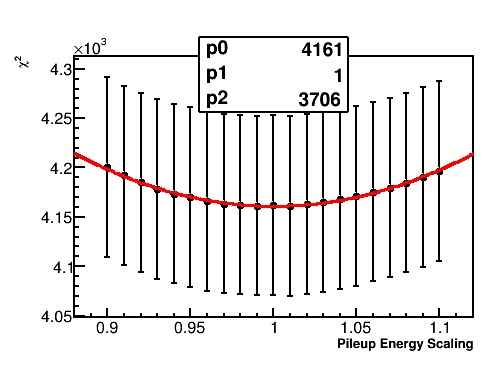
\includegraphics[width=\textwidth]{FullRatio_Chi2_Vs_PileupEnergyScaling_Canv_9d}
        \caption{\chisq versus pileup energy scale. The parabolic fit equation used was $y = p_{2}(x - p_{1})^{2} + p_{0}.$}
    \end{subfigure}% %you need this % here to add spacing between subfigures
    \hspace{1cm}
    \begin{subfigure}[t]{0.45\textwidth}
        \centering
        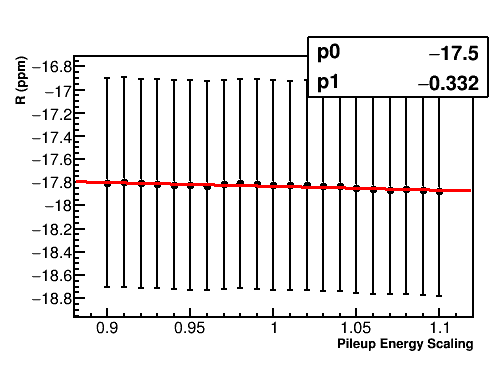
\includegraphics[width=\textwidth]{FullRatio_R_Vs_PileupEnergyScaling_Canv_9d}
        \caption{$R$ versus $C$. The parameter $p_{1}$ gives the sensitivity of $R$ to the value of $C$, with units in ppm.}
    \end{subfigure}
\caption[Pileup energy scale scan]{Scan over pileup energy scale. Data are from the 9d dataset.}
\label{fig:PEscan}
\end{figure}


\begin{table}
\centering
% \small
\setlength\tabcolsep{12pt}
\renewcommand{\arraystretch}{1.2}
\begin{tabular*}{0.65\linewidth}{@{\extracolsep{\fill}}lcccK}
% \begin{tabular}{@{\extracolsep{\fill}}lcccK}
  \hline
    \multicolumn{5}{c}{\textbf{Systematic Error due to Pileup Energy Scale}} \\
  \hline\hline
    Dataset & \multicolumn{1}{c}{$dR/dC$} & $\sigma_{C}$ & $C_{\text{min}}$ & \multicolumn{1}{c}{$\boldsymbol{\delta R}$} \\
  \hline
    60h & $-835.1$ & 0.023 & 0.997 & 19.4 \\
    HighKick & $-167.7$ & 0.022 & 0.995 & 3.7 \\
    9d & $-332.0$ & 0.016 & 1.000 & 5.5 \\ 
    Endgame & $-431.4$ & 0.012 & 0.982 & 5.3 \\
  \hline
\end{tabular*}
\caption[Systematic error due to fixed pileup energy scale factor]{Systematic error due to the fixed pileup energy scale parameter $C$ in the Ratio Method fits for the Run~1 precession frequency analysis. The bold column gives the systematic error on \R. Units for $dR/dC$ and $\delta R$ are in ppb.}
\label{tab:systematicError_pileupC}
\end{table}


\tabref{tab:PileupErrorsTotal} gives the quadrature sum for the total pileup systematic errors for the Run~1 precession frequency analysis datasets. As shown for each dataset the total error is below the target final error of \SI{40}{ppb} in spite of the contamination in the pileup shadow method. For future runs of the experiment with increased rate and therefore increased pileup, these errors may grow. In that case either the pileup shadow method might need to be improved to account for the contamination and pileup triplets, or discarded in favor of a different method.


\begin{table}
\centering
\setlength\tabcolsep{10pt}
\renewcommand{\arraystretch}{1.2}
\begin{tabular*}{\linewidth}{@{\extracolsep{\fill}}lcGGGG}
  \hline
    \multicolumn{6}{c}{\textbf{Total Pileup Systematic Errors}} \\
  \hline\hline
    Type of Error & Parameter & \multicolumn{1}{c}{60h} & \multicolumn{1}{c}{HighKick} & \multicolumn{1}{c}{9d} & \multicolumn{1}{c}{Endgame} \\
  \hline
    Amplitude & $P_{m}$  & 22.2 & 19.0 & 9.0  & 9.4 \\
    Phase     & $P_{t}$  & 17.6 & 19.0 & 17.1 & 14.3 \\
    Phase     & $C$      & 19.4 & 3.7  & 5.5  & 5.3 \\
  \hline
    Quadrature sum &  & 34.3 & 27.1 & 20.1 & 17.9 \\
  \hline 
\end{tabular*}
\caption[Total pileup-related systematic errors]{Total pileup systematic errors for the Run~1 precession frequency analysis datasets.}
\label{tab:PileupErrorsTotal}
\end{table}




\subsection{Gain systematic errors}
\label{sub:gainerror}


As described in \secref{sec:ReconWest}, the energies of the positron hits are gain-corrected for in-fill, short-term double pulse, and out-of-fill effects. The latter is largely temperature dependent and occurs over time scales much longer than a fill. This does not bias the precession frequency measurement as the phase is not time-dependent over the course of a fill. For the cases of in-fill or STDP gain variations, any uncorrected fluctuations in the gain causes an effective change in the energy threshold over the course of a fill which then modifies the average measured phase of the detected positrons. This causes a systematic shift in the extracted $R$ value. 


The IFG function as measured by the laser calibration system, \secref{sub:LaserCalibrationSystem}, describes the measured energies of the individual crystal hits as a function of time in-fill. It is given by \cite{IFG}
    \begin{align} \label{eq:IFG}
        E = E_{0}(1 - C_{A} e^{-t/\tau_{g}}),
    \end{align}
where $E_{0}$ is the `true' energy of the detected positron and $E$ is the measured energy. Constants $C_{A}$ and $\tau_{g}$ are measured with the laser calibration system, and then the function given in \equref{eq:IFG} is used to convert the measured energies back to their real energies. In order to determine a systematic error from the applied IFG function, the IFG function was re-applied to the crystal hits with modified parameters. Specifically, the amplitude of the IFG function $C_{A}$ and the lifetime $\tau_{g}$  were scanned over in multiplicative steps, separately, such that all crystal energies included in a cluster hit were adjusted by a multiplicative factor before re-summing. The multipliers applied to the IFG parameters were scanned over from 0 to 2 in steps of 0.25. The results of the scans for the 60h dataset are shown in \figref{fig:IFG_parameters}, with a comparison to the results from fits with the T-Method. It is immediately apparent that the sensitivities of the T-Method to the IFG parameters are significantly greater than that of the Ratio Method. The Ratio Method's insensitivity to slowly varying effects which it divides out is one of it's primary strengths. In fact, while there is an observable minimum in the T-Method \chisq results for the amplitude multiplier scan, no such minimum exists for the Ratio Method results.


% \begin{figure}
% \centering
%     \begin{subfigure}[]{0.45\textwidth}
%         \centering
%         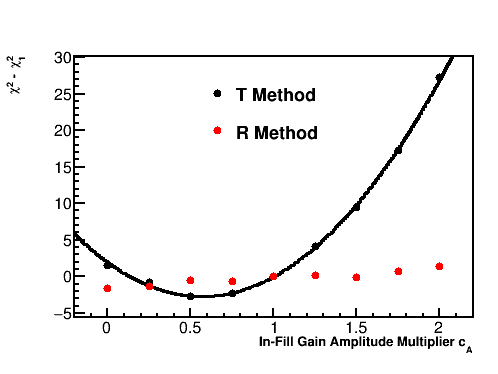
\includegraphics[width=\textwidth]{Chi2_Vs_IFG_Amp_crystals_compare_60h}
%         \caption{Normalized \chisq vs IFG amplitude multiplier. The T-Method points fit nicely to a parabolic curve while the Ratio Method points do not.}
%     \end{subfigure}% %you need this % here to add spacing between subfigures
%     \hspace{4mm}
%     \begin{subfigure}[]{0.45\textwidth}
%         \centering
%         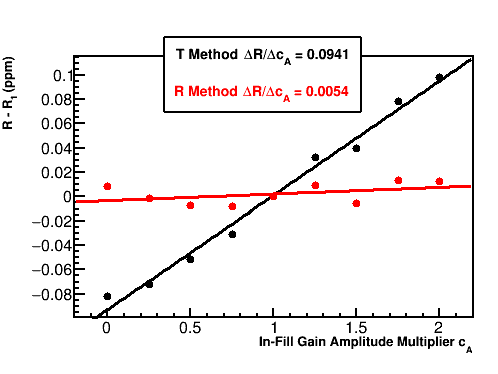
\includegraphics[width=\textwidth]{R_Vs_IFG_Amp_crystals_compare_60h}
%         \caption{$R$ values vs IFG amplitude multiplier. Both points are fit to straight lines, and the slopes are included in the text box in units of ppm.}
%     \end{subfigure}
% \caption[IFG amplitude multiplier scan]{Fitted \chisq's and $R$ values for the 60h dataset as a function of IFG amplitude multiplier. Results with ratio fits (red) are compared to T-Method fits (black). Values are normalized to their $C_{A} = 1$ results in order to put the curves on the same scale. As shown the sensitivity in the T-Method to the IFG amplitude is significantly larger than that of the Ratio Method. This is one of the primary strengths of the Ratio Method.}
% \label{fig:IFG_amplitude}
% \end{figure}


\begin{figure}
\centering
    \begin{subfigure}[]{0.45\textwidth}
        \centering
        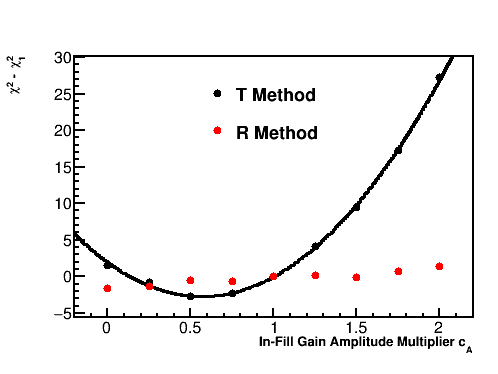
\includegraphics[width=\textwidth]{Chi2_Vs_IFG_Amp_crystals_compare_60h}
        \caption{Normalized \chisq vs IFG amplitude multiplier. The T-Method points fit nicely to a parabolic curve while the Ratio Method points do not.}
    \end{subfigure}% %you need this % here to add spacing between subfigures
    \hspace{4mm}
    \begin{subfigure}[]{0.45\textwidth}
        \centering
        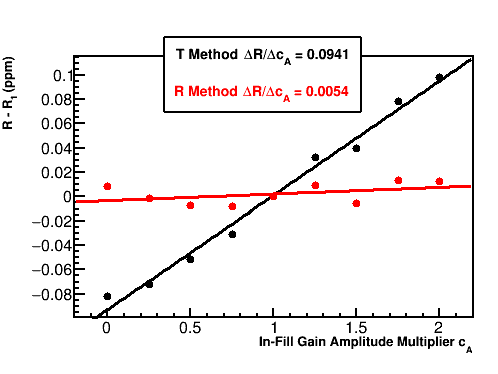
\includegraphics[width=\textwidth]{R_Vs_IFG_Amp_crystals_compare_60h}
        \caption{$R$ values vs IFG amplitude multiplier. Both points are fit to straight lines, and the slopes are included in the text box in units of ppm.}
    \end{subfigure}

    \begin{subfigure}[]{0.45\textwidth}
        \centering
        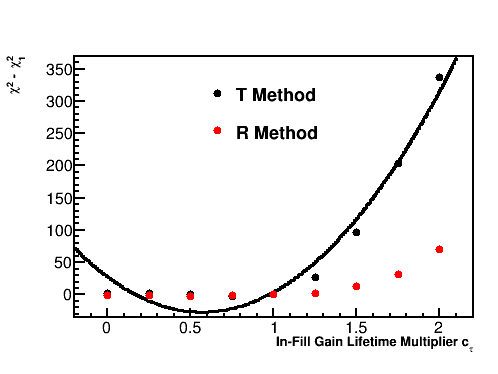
\includegraphics[width=\textwidth]{Chi2_Vs_IFG_Tau_crystals_compare_60h}
        \caption{Normalized \chisq vs IFG lifetime multiplier. Both T-Method and R-Method points flatten out at low multipliers, however the rise at high multipliers is larger for the T-Method.}
    \end{subfigure}% %you need this % here to add spacing between subfigures
    \hspace{4mm}
    \begin{subfigure}[]{0.45\textwidth}
        \centering
        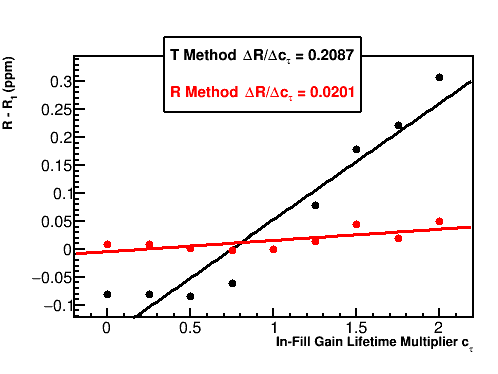
\includegraphics[width=\textwidth]{R_Vs_IFG_Tau_crystals_compare_60h}
        \caption{$R$ values vs IFG lifetime multiplier. Both points are fit to straight lines, and the slopes are included in the text box in units of ppm.}
    \end{subfigure}
\caption[IFG parameter systematic scan]{Fitted \chisq's and $R$ values for the 60h dataset as a function of IFG amplitude multiplier (top) and IFG lifetime multiplier (bottom). Results with ratio fits (red) are compared to T-Method fits (black). Values are normalized to their $C_{A} = 1$ and $C_{\tau} = 1$ results respectively in order to put the curves on the same scale. As shown the sensitivities in the T-Method to the IFG parameters are significantly larger than that in the Ratio Method. This is one of the primary strengths of the Ratio Method.}
\label{fig:IFG_parameters}
\end{figure}


Tables~\ref{tab:systematicError_IFG_amp} and \ref{tab:systematicError_IFG_tau} give the results for the IFG amplitude multiplier and lifetime multiplier scans respectively for the different datasets. Sensitivities for both the T-Method and Ratio Method fits are included. The uncertainties on the IFG parameters from fits to the laser data were in general of order 25\% \cite{AnnaPersonalComm}. This uncertainty multiplied against the as-measured Ratio Method sensitivities results in systematic errors of \SI{<6}{ppb} on the amplitude multiplier and \SI{<17}{ppb} for the lifetime multiplier for the various datasets. The individual numbers are given in column 5 of \tabref{tab:systematicError_IFG_amp} and column3 of \tabref{tab:systematicError_IFG_tau} respectively.


\begin{landscape}
\begin{table}
\centering
% \small
% \setlength\tabcolsep{12pt}
\renewcommand{\arraystretch}{1.2}
\begin{tabular*}{1\linewidth}{@{\extracolsep{\fill}}lccGKGGK}
  \hline
    \multicolumn{8}{c}{\textbf{Systematic Error due to IFG Amplitude}} \\
  \hline\hline
            & \multicolumn{1}{c}{T-Method} & \multicolumn{1}{c}{T-Method} & \multicolumn{1}{c}{R-Method} & \multicolumn{1}{c}{R-Method} & \multicolumn{1}{c}{R-Method} & \multicolumn{1}{c}{R-Method} & \multicolumn{1}{c}{R-Method} \\
    Dataset & \multicolumn{1}{c}{$dR/dC_{A}$} & \multicolumn{1}{c}{$C_{A_{\text{min}}}$} & \multicolumn{1}{c}{$dR/dC_{A}$} & \multicolumn{1}{c}{$\boldsymbol{\delta R}_{\sigma = 0.25}$} & \multicolumn{1}{c}{$\Delta R_{0x}$} & \multicolumn{1}{c}{$\Delta R_{2x}$} & \multicolumn{1}{c}{$\boldsymbol{\delta R}_{\text{max - 0x/2x}}$} \\
  \hline
    60h & 94.1 & 0.57 & 5.4 & 1.4 & 8.2 & 12.4 & - \\
    HighKick & 69.5 & 0.70 & -23.6 & 5.9 & 28.6 & -16.0 & 28.6 \\
    9d & 64.9 & 0.27 & 1.4 & 0.4 & -2.5 & -3.9 & - \\
    Endgame & 96.2 & 0.19 & 22.7 & 5.7 & -6.9 & 43.6 & 43.6 \\
  \hline
\end{tabular*}
\caption[Systematic error due to IFG amplitude]{Sensitivities and systematic errors for the IFG amplitude. T-Method sensitivities are included for comparison, along with the \chisq minima. Also included are changes in $R$ for fits with IFG amplitude multipliers of 0x and 2x. Systematic error columns are in bold, where the one on the left corresponds to the Ratio Method sensitivity multiplied by a 25\% uncertainty in the amplitude, and the one on the right corresponds to the absolute value of the maximum change in $R$ with the 0x and 2x multipliers applied. Only the HighKick and Endgame values are used from the column on the far right. Units for errors and sensitivities are in ppb.}
\label{tab:systematicError_IFG_amp}
\end{table}
\end{landscape}


\begin{table}
\centering
% \small
% \setlength\tabcolsep{12pt}
\renewcommand{\arraystretch}{1.2}
\begin{tabular*}{1\linewidth}{@{\extracolsep{\fill}}lcGKG}
  \hline
    \multicolumn{5}{c}{\textbf{Systematic Error due to IFG Lifetime}} \\
  \hline\hline
            & \multicolumn{1}{c}{T-Method} & \multicolumn{1}{c}{R-Method} & \multicolumn{1}{c}{R-Method} & \multicolumn{1}{c}{R-Method} \\
    Dataset & \multicolumn{1}{c}{$dR/dC_{\tau}$} & \multicolumn{1}{c}{$dR/dC_{\tau}$} & \multicolumn{1}{c}{$\boldsymbol{\delta R}_{\sigma = 0.25}$} & \multicolumn{1}{c}{$\Delta R_{0x}$} \\
  \hline
    60h & 208.7 & 20.1 & 5.0 & 8.2 \\
    HighKick & 114.7 & -44.8 & 11.2 & 28.6 \\
    9d & 81.7 & -46.4 & 11.6 & -2.5 \\
    Endgame & 207.3 & 66.1 & 16.5 & -6.9 \\
  \hline
\end{tabular*}
\caption[Systematic error due to IFG lifetime]{Sensitivities and systematic errors for the IFG lifetime. T-Method sensitivities are included for comparison. The systematic error columns is in bold, where the error corresponds to the Ratio Method sensitivity multiplied by a 25\% uncertainty in the lifetime. Units for errors and sensitivities are in ppb. The negative slope seen in the 9d dataset is somewhat of a mystery, for which no known issues might be responsible at the time of writing.}
\label{tab:systematicError_IFG_tau}
\end{table}


Examining \tabref{tab:systematicError_IFG_amp} in more detail however, some interesting features can be seen. The T-Method results, while not the primary subject of this analysis, nevertheless vary between the datasets, in that the scan minima are not consistent with one another. For the Ratio Method results, the HighKick and Endgame datasets exhibit greater sensitivities to the IFG amplitude than the 60h and 9d datasets. The HighKick dataset can be seen to have a negative sensitivity compared to the positive sensitivities of the other datasets, and the T-Method sensitivities for all datasets. The Endgame dataset has a greater sensitivity stemming from the fact that fits to the multiplicative factors of $C_{A} = 1.75$ and $C_{A} = 2$ produced noticeably better \chisq's and higher $R$ values, $\mathcal{O}(\SI{40}{ppb})$. These fits pulled the slope up from what is otherwise a very flat fit to the rest of the points, and imply that the default IFG multiplier should be greater than 1.


These various peculiarities imply there are imperfections in the gain corrections which have not been fully accounted for. Indeed recent investigations into the applied gain corrections show that for the HighKick and Endgame datasets the out-of-fill corrections were improperly applied during data production \cite{GainOscEndgameHighKick}. While this does not introduce a systematic uncertainty as a function of time in-fill as described before, it does shift the scale of the correction and by extension the extracted $R$ value. In order to determine more conservative bounds on the systematic errors to account for these deficiencies, the absolute changes in $R$ for the 0x and 2x multiplier fits were examined. These values are included in \tabref{tab:systematicError_IFG_amp}. The maximum of the two values was then taken as the systematic error on $R$ due to the IFG amplitude. In general the systematic errors as calculated from the maximum of the 0x or 2x fits are an order of magnitude larger than those errors calculated directly from the sensitivities. Because the scale of these numbers is still small compared to the Run~1 statistical errors however, they are deemed acceptable for this analysis. 

As for the lifetime multiplier scan results, it was observed that the \R and \chisq plots flattened out for small lifetimes as compared to large lifetimes, with no identifiable minima in the scan results. \R was seen to change by very little when the lifetime was small, as shown in the far right column of \tabref{tab:systematicError_IFG_tau}. Because of the larger changes in \R with the larger lifetimes, the sensitivities in the table were pulled to greater values than they otherwise might be. The choice was made to keep these large sensitivities in and use them in the calculation of the systematic error for a conservative approach, again justified by the gain issues mentioned previously.

In the calculation of the combined systematic error due to the IFG function parameters, the amplitude and lifetime parameter errors are added in quadrature, conservativley ignoring correlations between the two parameters in the fits to the laser data. Because the two parameters are correlated to a large degree, the 0x and 2x lifetime numbers were not used in the calculation of the HighKick and Endgame lifetime systematic errors as they have already been conservatively treated in the amplitude part of the error. The confidence in the scale of the Ratio Method results is ultimately preserved from the fact that the Ratio Method fits are not as sensitive to the gain variations as the T-Method fits, as the gain effects divide out. Going forward towards the end of the Run~1 analysis, once the outstanding gain issues have been resolved the systematic errors will be calculated directly from the sensitivities in all cases.


% , and in general the order of the out-of-fill and STDP corrections may be switched \cite{WhosOnFirst}. 
% the latter was shown to have a near-negligible effect on the final fitted $R$ value, of order \SI{20}{ppb}.


% \begin{landscape}
% \begin{table}
% \centering
% % \small
% % \setlength\tabcolsep{12pt}
% \renewcommand{\arraystretch}{1.2}
% \begin{tabular*}{1\linewidth}{@{\extracolsep{\fill}}lccGKGGK}
%   \hline
%     \multicolumn{8}{c}{\textbf{Systematic Error due to IFG Lifetime}} \\
%   \hline\hline
%             & \multicolumn{1}{c}{T-Method} & \multicolumn{1}{c}{T-Method} & \multicolumn{1}{c}{R-Method} & \multicolumn{1}{c}{R-Method} & \multicolumn{1}{c}{R-Method} & \multicolumn{1}{c}{R-Method} & \multicolumn{1}{c}{R-Method} \\
%     Dataset & \multicolumn{1}{c}{$dR/dC_{\tau}$} & \multicolumn{1}{c}{$C_{\tau_{\text{min}}}$} & \multicolumn{1}{c}{$dR/dC_{\tau}$} & \multicolumn{1}{c}{$\boldsymbol{\delta R}_{\sigma = 0.25}$} & \multicolumn{1}{c}{$\Delta R_{0x}$} & \multicolumn{1}{c}{$\Delta R_{2x}$} & \multicolumn{1}{c}{$\boldsymbol{\delta R}_{\text{max - 0x/2x}}$} \\
%   \hline
%     60h & 208.7 & 0.57 & 20.1 & 5.0 & 8.2 & 50.4 & - \\
%     HighKick & 114.7 & 0.58 & -44.8 & 11.2 & 28.6 & -32.7 & 32.7 \\
%     9d & 81.7 & 0.53 & -46.4 & 11.6 & -2.5 & -101.6 & - \\
%     Endgame & 207.3 & 0.53 & 66.1 & 16.5 & -6.9 & 108.4 & 108.4 \\
%   \hline
% \end{tabular*}
% \caption[Systematic error due to IFG lifetime]{Sensitivities and systematic errors for the IFG lifetime. T-Method sensitivities are included for comparison, along with the \chisq minima. Also included are changes in $R$ for fits with IFG amplitude multipliers of 0x and 2x. Systematic error columns are in bold, where the one on the left corresponds to the Ratio Method sensitivity multiplied by a 25\% uncertainty in the amplitude, and the one on the right corresponds to the absolute value of the maximum change in $R$ with the 0x and 2x multipliers applied. Only the HighKick and Endgame values are used from the column on the far right. Units for errors and sensitivities are in ppb.}
% \label{tab:systematicError_IFG}
% \end{table}
% \end{landscape}





The STDP correction is similay in many to the IFG correction \cite{STDP}. This correction is applied to pulses close in time, $\mathcal{O}(\text{ns})$, and is applied to the energies of the pulses before the in-fill gain correction. For the systematic error on $R$ due to the application of the STDP gain correction, a new production of the 60h dataset was processed without the STDP correction applied. Because of how the time-randomization is applied to the clusters in this analysis, a new version of the same dataset by default uses a different default randomization to the cluster times and the ratio histogram filling. As shown in \secref{sub:randomSeedFits}, the width in the fitted $R$ values for many random seeds is of order $\mathcal{O}(\SI{100}{ppb})$ making direct ratio fit comparisons between the two datasets un-informative. In order to avoid this difficulty, fits were done with the T-Method, and cluster times were randomized per-fill rather than per-cluster. Since the per-fill randomization uses fill ID's as the seeds for the randomization, and because the T-Method does not split the data into sub-datasets as the Ratio Method does, the randomization between the 60h dataset with and without the STDP correction is identical. The change in $R$ for T-Method fits with and without this correction is then taken as the upper bound on the systematic error for the inclusion of the STDP in the Ratio Method fits. This is reasonable as the previous IFG systematic studies showed a reduction in sensitivity to gain effects which is reasonably extended to the STDP correction error. \tabref{tab:systematicError_STDP} gives the T-Method fit results with and without the STDP, along with the change in $R$. This difference was found to be \SI{11.0}{ppb}, which is then taken as the systematic error for all datasets.


\begin{table}
\centering
% \small
% \setlength\tabcolsep{12pt}
\renewcommand{\arraystretch}{1.2}
\begin{tabular*}{1\linewidth}{@{\extracolsep{\fill}}lccK}
% \begin{tabular}{@{\extracolsep{\fill}}lcccK}
  \hline
    \multicolumn{4}{c}{\textbf{Systematic Error due to STDP}} \\
  \hline\hline
    Fit Type & \multicolumn{1}{c}{$R$ with STDP (ppm)} & \multicolumn{1}{c}{$R$ without STDP (ppm)} & \multicolumn{1}{c}{$\boldsymbol{\delta R}$ (ppb)} \\
  \hline
    T-Method & $-20.1619$ & $-20.1729$ & 11.0 \\
    % R-Method & -20.2041 & -20.1915 & -12.6 \\
  \hline
\end{tabular*}
\caption[Systematic error due to STDP]{T-Method fit results with and without the STDP gain correction on the 60h dataset. T-Method fits were done instead of Ratio Method fits in order to force the cluster-time randomization to be consistent between the two dataset productions. The change in $R$ in the bold column is taken as the upper bound on the systematic error in the Ratio Method due to the STDP gain correction.}
\label{tab:systematicError_STDP}
\end{table}

% I saw a change in R for the ratio method that was 12.6 ppb the other way, but the p values were very differnt and so I think it's just coincidence, because I expect the ratio method randomization to change the value by a lot


\tabref{tab:GainErrorsTotal} gives the quadrature sum for the total gain systematic errors for the Run~1 precession frequency analysis datasets. As shown for the 60h and 9d datasets the total error is below the target final error of \SI{20}{ppb}. For the HighKick and Endgame datasets, the errors are slightly larger than \SI{20}{ppb}, and should reduce once their known issues have been resolved. It should be noted that there is further evidence of the need for a correction for some type of residual gain effect which is somehow unmeasurable by the laser system \cite{AFThesis,SweigartEndgameOddities}\footnote{This implies the effect is very small.}. This combined with the previously mentioned issues in the Endgame and HighKick datasets warrant re-evaluations of the gain systematic errors once the final datasets are available. It is expected that the errors given here are reasonable approximations of the final errors, especially due to the Ratio Method's insensitivity to the gain relative to the T-Method. As a reminder, the errors given here, even with the crude approximations, are small compared to the statistical errors of the various datasets.



\begin{table}
\centering
\setlength\tabcolsep{10pt}
\renewcommand{\arraystretch}{1.2}
\begin{tabular*}{\linewidth}{@{\extracolsep{\fill}}lGGGG}
  \hline
    \multicolumn{5}{c}{\textbf{Total Gain Systematic Errors}} \\
  \hline\hline
    Type of Error & \multicolumn{1}{c}{60h} & \multicolumn{1}{c}{HighKick} & \multicolumn{1}{c}{9d} & \multicolumn{1}{c}{Endgame} \\
  \hline
    IFG amplitude  & 1.4 & 28.6 & 0.4 & 43.6 \\
    IFG lifetime  & 5.0 & 11.2 & 11.6 & 16.5 \\
    STDP  & 11.0 & 11.0 & 11.0 & 11.0 \\
  \hline
    Quadrature sum & 12.2 & 32.6 & 16.0 & 47.9 \\
  \hline 
\end{tabular*}
\caption[Total gain-related systematic errors]{Total gain-related systematic errors for the Run~1 precession frequency analysis datasets. Units are in ppb.}
\label{tab:GainErrorsTotal}
\end{table}





\subsection{CBO systematic errors}
\label{sub:cboerror}


If the CBO is mis-modeled then there will be a systematic error on $R$ since there is a an early-to-late change in both the frequency and the scale of the CBO. The CBO model is largely constrained by tracker measurements, but systematic errors can be evaluated by modifying the fixed frequency function given in \equref{eq:CBOfreqForm}, and the decoherence envelope of the CBO.

\tabref{tab:CBOFrequencyParameters} gives the CBO frequency model parameters for both tracker stations. The station 12 values are by default used in all fits to the data. Fits were performed with the station 18 values, and the changes in $R$ are given in \tabref{tab:systematicError_Station18}. The absolute values of the changes for the different datasets are conservatively taken as the systematic error on $R$ due to the choice of fixed CBO frequency model parameters. While the CBO parameters in the tracking analysis fits do have errors on the parameters, they are tiny compared to the systematic errors between the two tracker stations \cite{CBOFreqTrackingElog}. Some few fits were made by varying the fixed frequency parameters by $1\sigma$ in their individual respective errors, and the changes in $R$ were found to be negligible. For this reason the systematic errors from using station 18 values are taken as the errors.



\begin{table}
\centering
% \small
% \setlength\tabcolsep{10pt}
\renewcommand{\arraystretch}{1.2}
\begin{tabular*}{0.75\linewidth}{@{\extracolsep{\fill}}lH}
  \hline
    \multicolumn{2}{c}{\textbf{Change in $R$ with station 18 CBO parameters}} \\
  \hline\hline
    Dataset & \multicolumn{1}{c}{$\boldsymbol{\delta R}$} \\
  \hline
    60h & 7.5 \\
    HighKick & 0.4 \\
    9d & -2.0 \\
    Endgame & 8.0 \\
  \hline
\end{tabular*}
\caption[Changes in $R$ with tracker station 18 CBO frequency model parameters]{Changes in the fitted $R$ values with tracker station 18 CBO frequency model parameters instead of tracker station 12. The systematic errors are conservatively taken as the absolute value in the changes in $R$. Units are in ppb.}
\label{tab:systematicError_Station18}
\end{table}


The shape of the CBO, or the decoherence envelope, is also similarly constrained by the tracking analysis. The envelope by default is taken to be an exponential as given in \equref{eq:Ncbo} and shown in \figref{fig:CBOFreqAmp}. The other envelope which could reasonably exist in the data upon inspection in the tracking analysis is an exponential plus a constant
    \begin{align}
        e^{-t/\boldsymbol{\tau_{cbo}}} \rightarrow e^{-t/\boldsymbol{\tau_{cbo}}} + \boldsymbol{C},
    \end{align}
where $C$ is some constant CBO amplitude which persists over the course of the fill. In order to assess this systematic error, this new envelope was introduced into the $N_{cbo}(t)$ fit term. Fits were done with $C$ floating, where the starting values for $C$ in the Ratio Method fits were taken from T-Method fits to the data\footnote{T-Method starting values for $C$ were taken to be 0 which resulted in well-converging fits.}. While in T-Method fits the $C$ parameter converged to values with errors about half the value, in general in the Ratio Method fits the $C$ parameters had relatively large errors. In spite of the large errors however, the fits converged properly with the floating $C$ parameter. In general the final fit parameters are largely the same, with the exception being the fitted CBO lifetime and amplitude on the $N_{cbo}(t)$ term which both abouth halved. This is unsurprising as the lifetime is highly correlated to the amplitude. Only in the 9d dataset did some small complications arise, where the fit didn't particularly handle the floating $C$ parameter well. Fixing the lifetime to a value of \mus{99}, chosen such that the lifetime reduction was somewhat comparable to that seen in the HighKick dataset which had the same $n$ value, the $C$ parameter converged to a value close to and consistent with zero.

% Only in the 9d dataset did some small complications arise, where the CBO lifetime had to be fixed in order to get the fit to converge properly. In spite of this constraint it was found that the $C$ parameter converged to a negative value in the 9d dataset with a larger change in $R$. A reasonable hypothesis for this is that the correlations in the fitted parameters allows for good fits with varying fit values, and this fit just so happened to end up on a negative value. Regardless, though peculiar, the fit preference was clear and converged properly so result was taken to be acceptable.

The fitted values for the $C$ constants and the changes in the final fitted $R$ values are given in \tabref{tab:systematicError_CBOEnvelope}. As shown the changes in $R$ are of order 10s of ppb for some of the datasets, with $R$ varying both positively and negatively. These changes in $R$ are conservatively taken as the systematic errors on $R$ for the different datasets.


% Constraining the CBO lifetime and amplitude to smaller values does make the fit converge where C becomes a value similar to the other datasets - everything looks fine except then R is 100 ppb different. There is a weird step change if I step over the CBO lifetime. Not sure what this all implies, maybe that the CBO model is wrong in some way.



\begin{table}
\centering
% \small
% \setlength\tabcolsep{10pt}
\renewcommand{\arraystretch}{1.2}
\begin{tabular*}{0.75\linewidth}{@{\extracolsep{\fill}}lGGG}
  \hline
    \multicolumn{4}{c}{\textbf{Systematic Error due to CBO Envelope}} \\
  \hline\hline
    Dataset & \multicolumn{1}{c}{$C \times 10^{-4}$} & \multicolumn{1}{c}{$\sigma_{C} \times 10^{-4}$} & \multicolumn{1}{c}{$\boldsymbol{\delta R}$} \\
  \hline
    60h & 10.7 & 8.3 & 17.6 \\
    HighKick & 11.6 & 10.4 & -18.0 \\
    % 9d & -13.5 & 12.2 & 28.7 \\
    9d & -2.1 & 11.1 & 9.3 \\
    Endgame & 10.7 & 4.0 & -4.3 \\
  \hline
\end{tabular*}
\caption[Systematic error due CBO envelope]{Systematic error on $R$ due to the choice of CBO envelope. The fitted floating parameter $C$ and it's error are given along with the change in $R$ compared to the standard exponential envelope in units of ppb.}
\label{tab:systematicError_CBOEnvelope}
\end{table}



\tabref{tab:CBOErrorsTotal} gives the quadrature sum for the total CBO systematic errors for the Run~1 precession frequency analysis datasets. As shown for each dataset the total error is below the target final error of \SI{30}{ppb}. For future runs of E989 with more statistics it will be a question of whether the scale of these errors remains consistent or not. The changing frequency of the CBO in Run~1 was eliminated in Run~2, implying a reduction in any associated systematic errors. The increased statistics combined with the tracking analysis should constrain measurements of the CBO decoherence envelope even further, similarly reducing any associated systematic errors. On the other side of the coin, increased statistics might bring out higher order CBO effects which require improved modeling.


% should I cite and talk about David's new cbo model here?


\begin{table}
\centering
\setlength\tabcolsep{10pt}
\renewcommand{\arraystretch}{1.2}
\begin{tabular*}{\linewidth}{@{\extracolsep{\fill}}lGGGG}
  \hline
    \multicolumn{5}{c}{\textbf{Total CBO Systematic Errors}} \\
  \hline\hline
    Type of Error & \multicolumn{1}{c}{60h} & \multicolumn{1}{c}{HighKick} & \multicolumn{1}{c}{9d} & \multicolumn{1}{c}{Endgame} \\
  \hline
    CBO Frequency Model   & 7.5 & 0.4 & 2.0 & 8.0 \\
    % CBO Decoherence Envelope  & 17.6 & 18.0 & 28.7 & 4.3 \\
    CBO Decoherence Envelope  & 17.6 & 18.0 & 9.3 & 4.3 \\
  \hline
    % Quadrature sum & 19.1 & 18.0 & 28.8 & 9.1 \\
    Quadrature sum & 19.1 & 18.0 & 9.5 & 9.1 \\
  \hline 
\end{tabular*}
\caption[Total CBO-related systematic errors]{Total CBO-related systematic errors for the Run~1 precession frequency analysis datasets.}
\label{tab:CBOErrorsTotal}
\end{table}





\subsection{Lost muon systematic errors}
\label{sub:lostmuonserror}


Systematic errors from lost muons arise due to the fact that muons are preferentially lost at early times. Uncertainties in the lost muon spectrum itself, the fixed \K parameter in the Ratio Method fits, and any error due to phase differences between lost and stored muons are evaluated here.


As mentioned in \secref{subsec:lostmuons}, the triples spectrum is made with cuts as defined in \tabref{tab:lostmuoncuts}. Various backgrounds are subtracted off the triples spectrum in order to generate a clean sample of lost muons. \tabref{tab:lostmuonsvariousfits} gives the change in \R for various sets of cuts and background subtractions for the 9d and Endgame datasets. As shown the various different backgrounds and cuts ultimately make very little difference in the final fitted \R value. Similarly, stable beam contaminants in the form of deuterons and protons contaminate the lost muon spectrum. The former are largely removed by straightforward \DT and $\Delta t_{13}$ cuts. The latter can be mostly removed by cutting on the negative side of the $\Delta t_{13}$ distribution with $\Delta t_{13} \leq \SI{12.5}{ns}$ which separates the populations more readily, \figref{fig:deltaT13}. While this does largely remove the protons at the cost of statistics, the fitted \K parameter simply grows larger to compensate. Ultimately the effect on \R is negligible, with $\Delta R = \SI{-0.3}{ppb}$. The sum of these separate types of errors is conservatively taken at \SI{0.5}{ppb} for all datasets\footnote{For the T-Method fits, though the changes in \R are noticeably larger with the various cuts, they are still the same order of magnitude and the error is conservatively below \SI{1}{ppb}.}.


\begin{table}
\centering
\setlength\tabcolsep{10pt}
\renewcommand{\arraystretch}{1.2}
\begin{tabular*}{1\linewidth}{@{\extracolsep{\fill}}lHcHc}
  \hline
    \multicolumn{5}{c}{\textbf{$\Delta R$ with Various Lost Muon Cuts}} \\
  \hline\hline
    & \multicolumn{2}{c}{9d Dataset} & \multicolumn{2}{c}{Endgame Dataset} \\
  \hline
    Type of fit or cut & \multicolumn{1}{c}{$\Delta R$ (ppb)} & \K & \multicolumn{1}{c}{$\Delta R$ (ppb)} & \K \\
  \hline
    Default cuts & 0 & 2.510 & 0 & 2.345 \\
    No quadruple subtraction & 0.2 & 1.811 & -0.1 & 1.717 \\
    No accidental subtraction & 0.1 & 2.503 & <0.1 & 2.339 \\
    $\Delta t_{13} \leq \SI{12.5}{ns}$ & 0.1 & 4.469 & -0.3 & 4.248 \\
    $\SI{5}{ns} \leq \Delta t_{12, 23} \leq \SI{8.5}{ns}$ & 0.1 & 2.507 & <0.1 & 1.709 \\
    $\SI{100}{\MeV} \leq E_{1,2,3} \leq \SI{500}{\MeV}$ & <0.1 & 2.253 & <0.1 & 2.090 \\
  \hline 
\end{tabular*}
\caption[Effect on fitted R value due to lost muon cuts in the 9d and Endgame datasets]{Effect on the fitted \R value in the 9d and Endgame datasets with various cuts used or backgrounds subtracted. Also included are the various corresponding \K values which compensate for the level of statistics contained within $L(t)$ due to the differing cuts. Ultimately how the muon loss spectrum $L(t)$ is created has little bearing on the final fitted \R value.}
\label{tab:lostmuonsvariousfits}
\end{table}


\begin{figure}
    \centering
    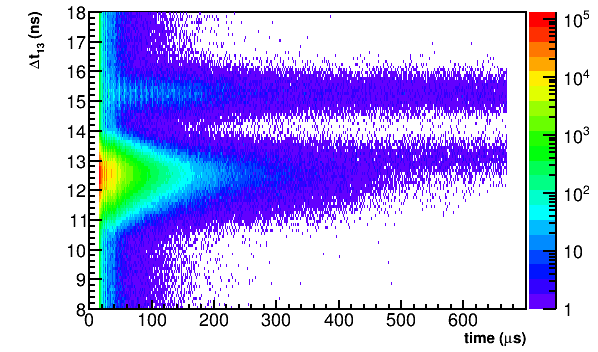
\includegraphics[width=.8\textwidth]{deltaT13_timeInFill_noCuts_Endgame}
    \caption[Lost muon $\Delta t_{13}$ distribution as a function of time in-fill]{Lost muon $\Delta t_{13}$ distribution as a function of time in-fill. The band of hits centered above \ns{15} corresponds to the deuteron contamination, while the band of hits centered above \ns{13} corresponds to the proton contamination.}
    \label{fig:deltaT13}
\end{figure}


Because \K is fixed in the Ratio Method fits from corresponding T-Method fits, the statistical correlation to $R$ is neglected and a systematic error must be estimated. The systematic error can be determined by scanning over the value of \K as in \figref{fig:kappaLossScan}. The error on \K is taken as the statistical error determined in the T-Method fit to the same data. \tabref{tab:systematicError_kappaLoss} gives the systematic errors on \R for the Run~1 precession frequency analysis datasets. As shown the systematic errors as calculated from the sensitivities are all small, $\delta R < \SI{5}{ppb}$. 


% However, as mentioned in \secref{sub:gainerror}, there were recently discovered issues in the applied gain corrections for the HighKick and Endgame datasets. Because the \K parameter is correlated to the gain, this implies the fitted \K values are wrong by a some amount for those datasets. In order to determine conservative errors due to the fixed \K parameter in those two cases, the \K values for the fits with 2x the IFG multiplier were used and compared to the default fits with 1x the IFG multiplier. The \K values for the HighKick and Endgame datasets with the 2x multiplier were 9.510 and 2.766 respectively. Compared to the default fit results of 5.651 and 2.345, these \K values are $11.1\sigma$ and $5.5\sigma$ away in terms of the T-Method statistical error. Multiplying the Ratio Method sensitivities by these larger errors gives the systematic errors in the far right column of \tabref{tab:systematicError_kappaLoss}. These alternative errors are an order of magnitude or so greater than the errors determined from the sensitivities, but are nevertheless still small compared to the Run~1 statistical errors. Once the final datasets have been created with the fixed gain parameters, the systematic errors will be re-evaluated. 
 
%Interestingly enough, though the Endgame dataset has the most lost muons, it is seen that the change in \R versus \K is larger in the other datasets. This is potentially due to the fact that \textbf{try to come up with something for this unless I can explain it away as an oddity.}


\begin{figure}
    \centering
    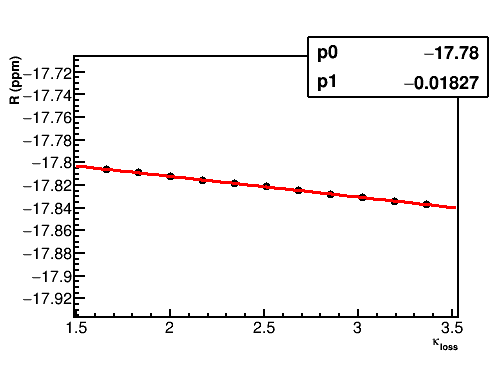
\includegraphics[width=.7\textwidth]{FullRatio_R_Vs_kappa_loss_Canv_9d}
    \caption[Scan over fixed \K]{The sensitivity of \R to the fixed \K parameter. Error bars have been removed from the plot. Units are in ppm, data are from the 9d dataset.}
    \label{fig:kappaLossScan}
\end{figure}


\begin{table}
\centering
% \small
% \setlength\tabcolsep{10pt}
\renewcommand{\arraystretch}{1.2}
\begin{tabular*}{0.75\linewidth}{@{\extracolsep{\fill}}lGcJG}
  \hline
    \multicolumn{5}{c}{\textbf{Systematic Error due to Fixed $\kappa_{loss}$}} \\
  \hline\hline
    Dataset & \multicolumn{1}{c}{$dR/d\kappa_{loss}$} & $\sigma_{\kappa_{loss}}$ & \multicolumn{1}{c}{$\boldsymbol{\delta R}$} & \multicolumn{1}{c}{$\Delta R_{\text{(w/ - w/o)}}$} \\
  \hline
    60h & -3.5 & 0.338 & 1.2 & -31.4 \\
    HighKick & -7.1 & 0.697 & 4.9 & -40.1 \\
    9d & -18.3 & 0.170 & 3.1 & -45.7 \\
    Endgame & -2.6 & 0.038 & 0.1 & -6.1 \\
  \hline
\end{tabular*}
\caption[Systematic error due to fixed $\kappa_{loss}$]{Systematic error due to the fixed $\kappa_{loss}$ parameter in the Ratio Method fits for the Run~1 precession frequency analysis datasets. All units are in ppb except for the $\sigma_{\kappa_{loss}}$ parameter which is unit-less. $\sigma_{\kappa_{loss}}$ comes from the T-Method fit results and scales with the number of statistics. The bold column gives the systematic errors on \R. The far right column gives the change in $R$ with the \K parameter in the fits versus without it entirely.}
\label{tab:systematicError_kappaLoss}
\end{table}


% \begin{table}
% \centering
% % \small
% % \setlength\tabcolsep{10pt}
% \renewcommand{\arraystretch}{1.2}
% \begin{tabular*}{\linewidth}{@{\extracolsep{\fill}}lGcJGK}
%   \hline
%     \multicolumn{6}{c}{\textbf{Systematic Error due to Fixed $\kappa_{loss}$}} \\
%   \hline\hline
%     Dataset & \multicolumn{1}{c}{$dR/d\kappa_{loss}$} & $\sigma_{\kappa_{loss}}$ & \multicolumn{1}{c}{$\boldsymbol{\delta R}$} & \multicolumn{1}{c}{$\Delta R_{\text{(w/ - w/o)}}$} &\multicolumn{1}{c}{$\boldsymbol{\delta R}_{2x-IFG}$} \\
%   \hline
%     60h & -3.5 & 0.338 & 1.2 & -31.4 & - \\
%     HighKick & -7.1 & 0.697 & 4.9 & -40.1 & 39.1 \\
%     9d & -18.3 & 0.170 & 3.1 & -45.7 & - \\
%     Endgame & -2.6 & 0.038 & 0.1 & -6.1 & 28.9 \\
%   \hline
% \end{tabular*}
% \caption[Systematic error due to fixed $\kappa_{loss}$]{Systematic error due to the fixed $\kappa_{loss}$ parameter in the Ratio Method fits for the Run~1 precession frequency analysis datasets. All units are in ppb except for the $\sigma_{\kappa_{loss}}$ parameter which is unit-less. $\sigma_{\kappa_{loss}}$ comes from the T-Method fit results and scales with the number of statistics. The bold columns gives the systematic errors on \R, where the one on the left corresponds to the systematic error as calculated from the sensitivity, and the one on the right corresponds to the systematic error for the HighKick and Endgame datasets using the \K value determined from fits with 2x the IFG multiplier.}
% \label{tab:systematicError_kappaLoss}
% \end{table}

% 21.1 for 60h using same procedure
% 134.2 for 9d using same procedure


The most dangerous potential systematic error has to due with the phases of the lost muons. If muon losses come from a population of muons with a different average phase than the stored muons, then there will be a phase shift over the course of a fill. This combined with the fact that muons are preferentially lost at early times implies the extracted \wa frequency will be systematically pulled. Simulation and data have shown a correlation between phase and momentum at injection \cite{HannahLossStudy,SudeshnaElbaTalk}. If the losses are momentum dependent and the phase-momentum correlation is preserved after injection, then there will be a systematic error. From simulation losses are momentum dependent \cite{MikeLosses}, the general idea being that the low kick applied in Run~1 resulting in an off-center stored muon beam results in more muons at greater radii with larger momentum near the edge of the storage aperture, compared to those muons on the inside of the storage region. The phase-momentum correlation originates from the fact that muons are born at different points within the accelerator beam-line before injection. Muons born at earlier locations in the beam-line will live longer within the magnetic field, during which their spins will precess and their \gmtwo phases change. Such muons could reasonably exist within a different injection parameter phase space, such that they exhibit larger betatron amplitudes once stored in the ring. Because losses most likely come from muons which oscillate to high betatron amplitudes, and for those muons at greater radii with larger momenta, such a systematic effect certainly exists, and thus an error needs to be estimated. Further simulation efforts are underway, along with data-driven studies, to understand and quantify the phase-momentum correlation and momentum-dependent loss probabilities \cite{MikeLosses,HannahLossStudy2}. Here is given an estimation of the muon loss phase bias systematic error using the author's own calculations for the losses for the different Run~1 datasets.


The systematic shift in \wa can be written as
    \begin{align}
        \frac{\Delta\omega_{a}}{\omega_{a}} = \frac{1}{\omega_{a}}\frac{d\langle\phi\rangle}{dt},
    \end{align}
where $d\langle\phi\rangle/dt$ is the change in average phase over the course of a fill. With some assumptions made with regards to stored and lost muon populations this can be written as \cite{MikeLosses}
    \begin{align} \label{eq:phaseChangeLostMuons}
        \frac{d\langle\phi\rangle}{dt} = f_{s} \cdot f_{l} \cdot \Delta\phi_{s-l},
    \end{align}
where $f_{s}$ is the fraction of stored muons to all muons, $f_{l}$ is the fractional loss rate, and $\Delta\phi_{s-l}$ is the phase difference between the stored and lost muon populations. The simulation studies in the afore-referenced document gives estimates of $f_{s} \approx 0.9$ and $\Delta\phi_{s-l} \approx \SI{1}{mrad}$. The fractional losses (the integral in \equref{eq:lambdalosses} times the final fitted $\kappa_{loss}$ parameter, assuming no losses are included in $L(t)$ before the fit start time) for the Run~1 precession frequency analysis datasets as determined in this analysis are shown in \figref{fig:fractionallosses}. As shown the losses rise sharply at early times before leveling off to a constant rate around \mus{100} into the fill. Taking the first \mus{70} of the fit and assuming the loss rate is constant over the course of the fill, the approximate loss rates for the different datasets can be determined\footnote{While the loss rate levels off after \mus{100}, losses occur mostly at early times, so this is a fine approximation.}. These are given in \tabref{tab:systematicError_lostMuonBias}. Applying the approximate loss probabilities into \equref{eq:phaseChangeLostMuons}, along with $\omega_{a} \approx \SI{1.44}{rad/\mus{}}$, the systematic shifts in the precession frequency are found. They are included in \tabref{tab:systematicError_lostMuonBias}.



\begin{figure}
    \centering
    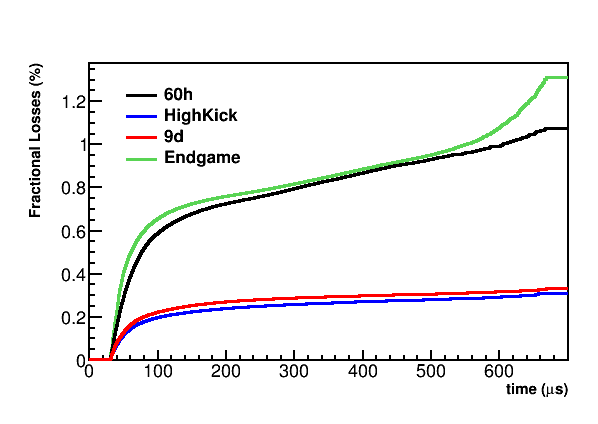
\includegraphics[width=.8\textwidth]{fractionalLosses_dataset_comparison}
    \caption[Fractional muon losses in the analyzed Run~1 datasets]{Fractional losses for the Run~1 precession frequency analysis datasets. The curves begin at \mus{30.2} which is where the fit begins. A value of 1\% at a specific time $t$ indicates that there are 1\% fewer stored muons at that time than there would be if there were no losses at all. The Endgame and 60h datasets can be seen to have the most losses, while the 9d and HighKick have less. This is due to the higher kicks in the latter datasets which put the stored muon beam on a more central orbit. The upward tail at the end of the Endgame dataset corresponds to the remnant proton contamination.}
    \label{fig:fractionallosses}
\end{figure}



\begin{table}
\centering
% \small
% \setlength\tabcolsep{10pt}
\renewcommand{\arraystretch}{1.2}
\begin{tabular*}{0.75\linewidth}{@{\extracolsep{\fill}}lccG}
  \hline
    \multicolumn{4}{c}{\textbf{Systematic Error due to Lost Muon Phase Bias}} \\
  \hline\hline
    Dataset & & $f_{l}$ (\%/\mus{70}) & \multicolumn{1}{c}{$\Delta\omega_{a}/\omega_{a}$ (ppb)} \\ 
  \hline
    60h & & 0.60 & -53.6 \\ 
    HighKick & & 0.20 & -17.9 \\
    9d & & 0.25 & -22.3 \\
    Endgame & & 0.65 & -58.0 \\
  \hline
\end{tabular*}
\caption[Systematic error due to lost muon phase bias]{Loss rates and associated shift in \wa for the Run~1 precession frequency analysis datasets. Loss rates are determined by inspection of the respective curves for the different datasets, and are approximate. The systematic shifts here are negative, due to the fact that the average phase of the stored muons is greater than that of lost muons, as determined in simulation.}
\label{tab:systematicError_lostMuonBias}
\end{table}


Taking the shifts in \wa as the systematic errors, the approximations here are on the order of \SI{50}{} -- \SI{60}{ppb} for the 60h and Endgame datasets, and on the order of \SI{20}{ppb} for the HighKick and 9d datasets. These estimates are the same order of magnitude as determined in other evaluations with slightly different parameters \cite{SudeshnaElbaTalk}. Estimates on the absolute upper bound of the systematic error is of order \SI{125}{ppb} \cite{AFThesis,MikeLosses}. As simulations improve and more studies are undertaken, the uncertainties here may be replaced in favor of actual corrections, in which case the systematic errors would then be the uncertainties in the evaluation of those corrections. While not below the target goal of \SI{20}{ppb}, the systematic errors listed here are nevertheless small compared to the Run~1 statistical errors, expected to decrease going forward in future runs.


\subsection{Ratio construction systematic errors}
\label{sub:TimeShiftingParameters}


In the construction of the ratio data, when filling the four sub-datasets as in \equref{eqn:fourHistsInText}, the parameters $T_{a}$ and $\tau_{\mu}$ for the \gmtwo period and muon lifetime need to be known a priori. If these parameters are incorrectly chosen, then it is possible there will be a systematic shift on $R$. This is especially important when considering $T_{a}$, because the quantity which the E989 experiment is measuring must be used in the analysis, creating a sort of self-dependence. The question then naturally arises as to how well the $T_{a}$ parameter needs to be known. As described in \secref{sub:ratio_method}, the input value for $T_{a}$ is nominally taken as the result from the E821 experiment. 

In order to determine systematic errors from these two fixed quantities, they were scanned over when forming the ratio data before fitting. The input value for $T_{a}$ was varied from \SI{-30}{ppm} to \SI{+30}{ppm} around the default value in steps of \SI{3}{ppm}. The input value for $\tau_{\mu}$ was varied from \SI{64.04}{\micro s} to \SI{64.84}{\micro s} in steps of \SI{0.04}{\micro s}. See \figref{fig:ratioConstructionParsScan} for scan results for the 60h dataset. See \tabref{tab:ratioConstructionParsScan} for the sensitivities determined from the scans for all datasets. As shown the sensitivities vary both positively and negatively for the different datasets, and are extremely small. The positive and negative variations imply there is no real systematic effect at play, and that as long as a reasonable choice for these two parameters is made, then the ratio data is very insensitive to the exact values chosen. 

In order to be conservative however, a scale for the changes in $R$ is given. Since the measured \gmtwo period in the data is already modified by the hardware blinding, it is technically the hardware shifted \gmtwo period that we want to use. The calorimeter digitizers use a ``40'' MHz clock which has been blinded to a value in the range of 39.997 to \SI{39.999}{MHz}\cite{ClockManual}. This corresponds to a 75 ppm range in the frequency, in a uniform distribution. Calculating the uncertainty from the uniform distribution and adding it in quadrature with a conservative \SI{10}{ppm} uncertainty in the guess on the true \gmtwo period from the E821 result, 
            \begin{align}
                \delta T_{a} = \sqrt{(75)^{2}/12 + 10^{2}} = \SI{23.8}{ppm}.
            \end{align}
This results in a change in $R$ on the order of \SI{2.4}{ppb} for the 60h and HighKick datasets, and less for the 9d and Endgame datasets. 

%Because this is so small and because the sensitivities vary positively and negatively, any systematic error from this quantity can reasonable be said to not exist.

Similarly, the sensitivities of $R$ to the chosen muon lifetime are very small, order \SI{}{ppb/ \micro s}. Since the uncertainties in the muon lifetime are of order \ns{} from fits to the data, any systematic errors from this parameter would be completely negligible even if the sensitivities all had the same sign.


\begin{figure}
\centering
    \begin{subfigure}[t]{0.45\textwidth}
        \centering
        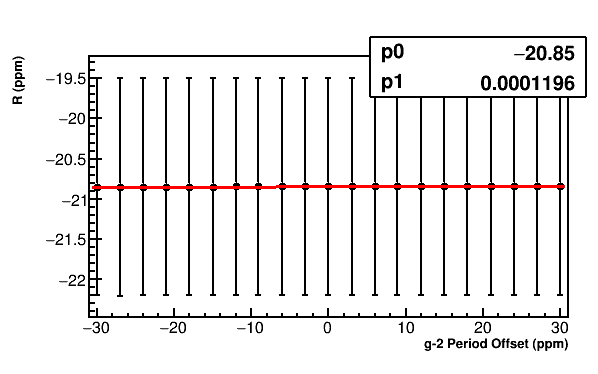
\includegraphics[width=\textwidth]{FullRatio_R_Vs_gm2PeriodGuess_Canv_60h}
        \caption{$R$ versus input value for $T_{a}$, where the x axis is given in units of a ppm level shift of the default choice for $T_{a}$.}
    \end{subfigure}% %you need this % here to add spacing between subfigures
    \hspace{4mm}
    \begin{subfigure}[t]{0.45\textwidth}
        \centering
        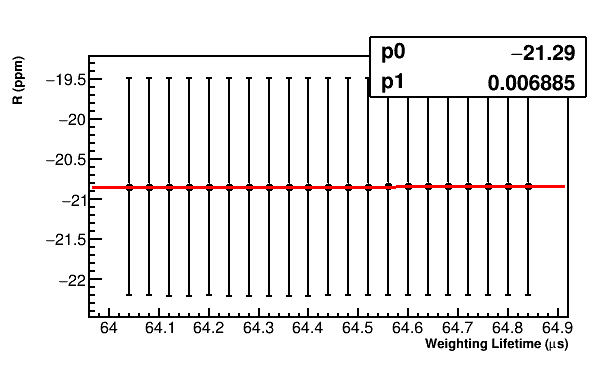
\includegraphics[width=\textwidth]{FullRatio_R_Vs_weightingLifetime_Canv_60h}
        \caption{$R$ versus the input value for $\tau_{\mu}$. Parameter $p_{1}$ gives the sensitivity in \SI{}{ppm/ \micro s}.}
    \end{subfigure}
\caption[Scans over ratio construction parameters]{Scans over ratio construction parameters for the 60h dataset. Error bars have been removed from the plots. In general the points are randomly spread around, and sensitivities are very small.}
\label{fig:ratioConstructionParsScan}
\end{figure}


\begin{table}
\centering
% \small
\setlength\tabcolsep{20pt}
\renewcommand{\arraystretch}{1.2}
\begin{tabular*}{0.7\linewidth}{@{\extracolsep{\fill}}lcHH}
% \begin{tabular}{@{\extracolsep{\fill}}lcccK}
  \hline
    \multicolumn{4}{c}{\textbf{Sensitivity to Ratio Construction Parameters}} \\
  \hline\hline
    Dataset & & \multicolumn{1}{c}{$dR/d_{T_{a}}$} & \multicolumn{1}{c}{$dR/d_{\tau_{\mu}}$} \\
  \hline
    60h & & 0.1 & 6.9 \\
    HighKick & & -0.1 & -4.1 \\
    9d & & <0.1 & -1.1 \\ 
    Endgame & & <0.1 & 0.6 \\
  \hline
\end{tabular*}
\caption[Sensitivities of $R$ to ratio construction parameters]{Sensitivities of $R$ to ratio construction parameters. $dR/d_{T_{a}}$ is in units of ppb/ppm, while $dR/d_{\tau_{\mu}}$ is in units of \SI{}{ppb/ \micro s}. In both cases the sensitivities are both extremely small, and vary negatively and positively for the different datasets.}
\label{tab:ratioConstructionParsScan}
\end{table}



\subsection{Binning systematic errors}
\label{sub:binning_systematic_errors}


When constructing the time spectra to be fit, bin widths and the starting edge of the bin are by default chosen to be \SI{149.2}{ns} and \SI{0}{ns} respectively. In order to verify that no systematics arise from the choice of these parameters, the values were scanned over. The bin width was scanned from \SI{148.7}{ns} to \SI{149.7}{ns} in steps of \SI{0.1}{ns}, while the bin edge was scanned from \SI{0}{ns} to \SI{149.2}{ns} in steps of \SI{14.92}{ns}. \figref{fig:binParametersScan} shows scan results for the 9d dataset. \tabref{tab:binParametersScan} gives the sensitivities of $R$ to both parameters. 

Upon general inspection of the fit points themselves, it was found that the trends weren't so convincing as the points varied relatively widely. Still a line was fit to the points to asses the scale of the changes. For the bin edge scan, it was verified that a shift of one bin width returned the same fit results as the default shift of \ns{0}. This combined with the negligible sensitivities and varying points implies no systematic effects on $R$ from the choice of bin edge. For the sensitivities to the choice of bin width, not only did the points vary, but the trends were both positive and negative depending on the dataset. In general the choice of bin width should be optimized to be equal to the peak of the cyclotron period distribution of the stored muons, which from the fast rotation analysis informed the choice of \SI{149.2}{ns}. Therefore it is reasonable to quote no systematic error for the choice of bin width. If one wanted to be conservative and quote a systematic error however, the sensitivities could be multiplied against the uncertainty in the optimal bin width. This uncertainty from the fast rotation analysis would certainly be less than \SI{0.1}{ns}, which would correspond to uncertainties of \SI{2.5}{}, \SI{0.6}{}, \SI{2.3}{}, and \SI{4.2}{ppb} for the 60h, HighKick, 9d, and Endgame datasets respectively, all of which are practically negligible.



\begin{figure}
\centering
    \begin{subfigure}[t]{0.45\textwidth}
        \centering
        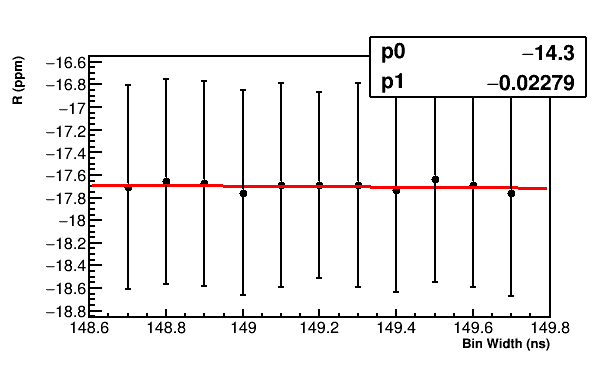
\includegraphics[width=\textwidth]{FullRatio_R_Vs_binWidth_Canv_9d}
        \caption{}
    \end{subfigure}% %you need this % here to add spacing between subfigures
    \hspace{1cm}
    \begin{subfigure}[t]{0.45\textwidth}
        \centering
        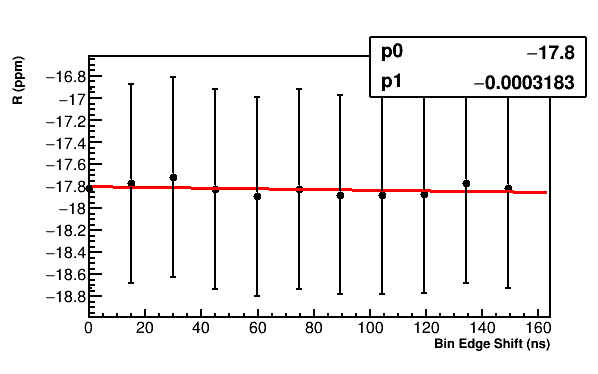
\includegraphics[width=\textwidth]{FullRatio_R_Vs_binEdgeShift_Canv_9d}
        \caption{}
    \end{subfigure}
\caption[Scans over binning parameters]{Scans over binning parameters for the 9d dataset. In general the points are randomly spread around, indicating no real systematic effect.}
\label{fig:binParametersScan}
\end{figure}


\begin{table}
\centering
% \small
\setlength\tabcolsep{20pt}
\renewcommand{\arraystretch}{1.2}
\begin{tabular*}{0.7\linewidth}{@{\extracolsep{\fill}}lGG}
% \begin{tabular}{@{\extracolsep{\fill}}lcccK}
  \hline
    \multicolumn{3}{c}{\textbf{Sensitivity to Binning Parameters}} \\
  \hline\hline
    Dataset & \multicolumn{1}{c}{$dR/d_{\text{bin width}}$} & \multicolumn{1}{c}{$dR/d_{\text{bin edge}}$} \\
  \hline
    60h & 24.5 & -0.1 \\
    HighKick & 6.0 & -0.7 \\
    9d & -22.8 & -0.3 \\ 
    Endgame & -41.7 & -0.6 \\
  \hline
\end{tabular*}
\caption[Sensitivities of $R$ to binning parameters]{Sensitivities of $R$ to binning parameters. Units are in ppb/ns. While some of these values may appear significant, inspection of the actual plots reveals that the actual trends are not quite so convincing.}
\label{tab:binParametersScan}
\end{table}



\subsection{Systematic error from differential decay}


Muons are injected into the storage ring with a range of momenta. Muons with larger momenta will in general live longer than muons with smaller momenta due to their time-dilated lifetimes. Muons at smaller radii therefore decay more often, leading to an increasing beam radial position and average momentum over the course of a fill. Decay positrons at greater radii with larger momenta in general take longer to reach calorimeters than those at small radii with smaller momenta. In the precession frequency measurement, the hit times of the detected positrons naturally correspond to offset times from when the muons decayed equal to the drift times. Because the average drift time changes over the course of a fill due to the average momentum distribution increase, there is thus a changing phase over the course of a fill. To add to that, as discussed in \secref{sub:lostmuonserror}, there is a phase-momentum correlation for muons at injection. This only compounds upon the changing phase even further. The systematic error due to this effect is called ``differential decay.'' 

Underway beam-line simulations are needed to fully measure the phase-momentum correlation and fully estimate this systematic error. A calculation for the previous E821 experiment resulted in a shift on \wa of $\langle \omega_{a} \rangle / \omega_{a} \approx \SI{-36.8}{ppb}$ \cite{DiffDecayJason}, which should be comparable to any calculation for E989. The level of the fully evaluated systematic shift may not be small compared to the final target systematic error goal, but for Run~1 the scale of this estimate is deemed to be acceptable. For the purposes of this document, an upper bound of \SI{40}{ppb} is taken as the systematic error. Because the differential decay effect only increases the average stored momentum of the beam and can't decrease it, a correction can be applied if any final uncertainty is deemed to be too large. 


% An estimation of the error neglecting the phase momentum correlation yielded a shift of \SI{-3.8}{ppb} \cite{DiffDecayMetodiev}. Finally, an estimation by a first principles approach gave a value of \SI{-12}{ppb} \cite{AFThesis}. 




\subsection{Systematic errors in the E-field and pitch corrections}
\label{sub:EfieldPitchErrors}


The electric field and pitch corrections modify the final value extracted for \wa as described in \secref{sec:corrections}. Any errors in the estimation of these corrections is by extension an error in the precession frequency measurement. The evaluation of these errors is performed by separate working groups. Given here are preliminary estimates of the errors. 


The pitch correction is evaluated by the tracking analysis and is dependent on the vertical width of the muon beam. A preliminary analysis of the 60h dataset calculated an estimated correction and systematic error of \cite{PitchReview,PitchElba}
    \begin{align} \label{eq:pitchError}
        C_{P} \sim -160 \pm \SI{15}{ppb}.
    \end{align}
This error is split into track reconstruction errors of which there are many $(\mathcal{O}(\SI{10}{ppb}))$, a tracker-calorimeter acceptance correction with a small expected error, and uncertainty in simulation models used in various parts of the tracking. While the actual correction itself may differ between datasets, the error in the correction is expected to be relatively consistent. The pitch correction error given in \equref{eq:pitchError} is taken as the systematic error for all datasets. 

% 16 ppb acceptance error


The E-field correction is evaluated with the fast rotation analysis and is dependent on the equilibrium radius of the muon beam. Analyses to the 60h, 9d, and Endgame datasets by the Cornell fast rotation analysis group yielded the results shown in \tabref{tab:EfieldCorrections}. While not the final numbers for Run~1, the estimates and errors given will change only slightly from further DQC cuts. For the HighKick dataset which has not been evaluated at the time of writing, a systematic error on the E-field correction is taken as the largest error from the other datasets, that being \SI{36}{ppb} for the 9d dataset.


\begin{table}
\centering
% \small
% \setlength\tabcolsep{20pt}
\renewcommand{\arraystretch}{1.2}
\begin{tabular*}{\linewidth}{@{\extracolsep{\fill}}lccc}
  \hline
    \multicolumn{4}{c}{\textbf{Electric field corrections}} \\
  \hline\hline
    Dataset & Correction & Statistical error & Systematic error \\
  \hline
    60h & $-463$ & 1.0 & 27.0 \\
    HighKick & N/A & N/A & N/A \\
    9d & $-463$ & 1.0 & 36.0 \\
    Endgame & $-467$ & 1.0 & 20.0 \\
  \hline
\end{tabular*}
\caption[Electric field corrections estimated by the Cornell fast rotation analysis group]{Electric field corrections estimated by the Cornell fast rotation analysis group \cite{AntoineEField60h,AntoineEField9d,AntoineEFieldEndgame}. Units are in ppb.}
\label{tab:EfieldCorrections}
\end{table}



The above corrections make certain assumptions with regards to the conditions which influence the stored beam dynamics. Further errors can be attributable to non-linearities in the electrostatic quadrupole field, misalignment of the quadrupole plates, the changing voltage on the quadrupole plates due to the bad resistors, and any residual radial magnetic field. Preliminary analyses using simulation have estimated additional systematic errors on the pitch and E-field corrections of \SI{\sim5}{ppb} and \SI{\sim20}{ppb} respectively \cite{DaveRubinElbaBadResistors,DaveRubinBadResistorsUpdate}. The error for the pitch correction was already included in the number given in \equref{eq:pitchError}, and the error for the E-field correction is conservatively added in quadrature with the errors given in \tabref{tab:EfieldCorrections}. Simulation efforts are continuing in order to identify and nail down these errors even further. While the errors listed here are greater than the target quadrature sum of \SI{30}{ppb}, they are nonetheless small compared to the statistical error on $R$ and are deemed acceptable for Run~1.


\subsection{Systematic error due to beam motion}


As described in \secref{sec:MuonBeamMeasurements}, the vertical position of the stored muon beam changes over the course of a fill. Because the \gmtwo phase is position dependent, this leads to a changing average phase and thus a systematic error. Preliminary studies fitting the average \gmtwo phase with the tracker data have calculated systematic shifts in \wa for the 60h and Endgame datasets of \SI{115}{} and \SI{180}{ppb} respectively \cite{BadResistorsVolodya}. Since these are one-directional shifts in \wa, similar to the differential decay effect, they can be applied as corrections to the final extracted precession frequency. As systematic studies mature and the shifts are better quantified, this is the intended action. For now these numbers are taken as limits on the systematic errors for their respective datasets, with the smaller number from the 60h dataset being applied to the HighKick and 9d datasets as well. The 60h result was chosen instead of the Endgame result because the Endgame dataset saw noticeably larger drift due to further degradation of the quadrupole resistors.




\subsection{Systematic error summary}

\textbf{make sure table is filled with all correct updated errors}

\tabref{tab:FinalSystematicErrors} gives all evaluated systematic errors in this analysis as described in the preceding sections. The final total quadrature sums of the systematic errors including the various preliminary and conservative estimates for some errors lie within the range \SI{140}{} -- \SI{200}{ppb}. These are in comparison to the final target goal of \SI{70}{ppb} for the precession frequency measurement. Once the gain issues are resolved and the other working groups improve their systematic uncertainty evaluations, the systematic errors for Run~1 and future runs of E989 will almost certainly reach the target goal. Indeed just removing the stored muon beam systematic error results in systematic errors in the range of \SI{70}{} -- \SI{100}{ppb}, much closer to the target of \SI{70}{ppb}. As the systematic errors stand currently in this analysis, they are all small compared to the Run~1 statistical errors of each respective dataset, making the presented analysis statistics-limited. 



\begin{table}
\centering
% \small
% \setlength\tabcolsep{10pt}
\renewcommand{\arraystretch}{1.2}
\begin{tabular*}{\linewidth}{@{\extracolsep{\fill}}lGGGG}
  \hline
    \multicolumn{5}{c}{\textbf{Run~1 Precession Frequency Systematic Errors}} \\
  \hline\hline
    Error & \multicolumn{1}{c}{60h} & \multicolumn{1}{c}{HighKick} & \multicolumn{1}{c}{9d} & \multicolumn{1}{c}{Endgame} \\ 
  \hline
    Pileup amplitude & 22.2 & 19.0 & 9.0 & 9.4 \\
    Pileup phase - time-shift & 17.6 & 19.0 & 17.1 & 14.3 \\
    Pileup phase - energy-scale & 19.4 & 3.7 & 5.5 & 5.3 \\
    In-fill gain amplitude & 1.4 & 28.6 & 0.4 & 43.6 \\
    In-fill gain lifetime & 5.0 & 11.2 & 11.6 & 16.5 \\
    STDP On/Off & \sim 11.0 & \sim 11.0 & \sim 11.0 & \sim 11.0 \\
    CBO frequency model & 7.5 & 0.4 & 2.0 & 8.0 \\
    CBO decoherence envelope & 17.6 & 18.0 & 9.3 & 4.3 \\
    Lost muon cuts & < 0.5 & < 0.5 & < 0.5 & < 0.5 \\
    Fixed \K & 1.2 & 4.9 & 3.1 & 0.1 \\
    Ratio construction $T_{a}$ & 2.4 & 2.4 & < 2.4 & < 2.4 \\
    Ratio construction $T_{\mu}$ & < 0.1 & < 0.1 & < 0.1 & < 0.1 \\
    Bin width & 2.5 & 0.6 & 2.3 & 4.2 \\
    % Bin edge & - & - & - & - \\
  \hline
    Quadrature Sum & 41.3 & 46.4 & 27.8 & 52.2 \\
  \hline\hline
    Lost muon phase bias & 53.6 & 17.9 & 22.3 & 58.0 \\
    Differential decay & < 40 & < 40 & < 40 & < 40 \\
    Pitch correction & 15 & \sim 15 & \sim 15 & \sim 15 \\
    E-field correction & 33.6 & \sim 41.2 & 41.2 & 28.3 \\
    Stored beam motion & \sim 115 & \sim 115 & \sim 115 & \sim 180 \\
  \hline
    Quadrature Sum & 138.0 & 130.6 & 131.3 & 195.9 \\
    Quadrature Sum * & 76.3 & 62.0 & 63.4 & 77.4 \\
  \hline\hline
    Total Quadrature Sum & 144.1 & 138.6 & 134.2 & 202.8 \\
    Total Quadrature Sum * & 86.8 & 77.4 & 69.2 & 93.3 \\
  \hline
\end{tabular*}
\caption[Systematic errors evaluated in the Run~1 precession frequency datasets]{Final systematic errors evaluated in the Run~1 precession frequency analysis to the 60h, HighKick, 9d, and Endgame datasets. All units are in ppb. The table is split into two sections. The upper section consists of systematic errors directly evaluated by the author while the lower section consists of preliminary systematic estimates by other working groups. The E-field and pitch correction errors have been added in quadrature with the quadrupole errors. The publication errors for the Run~1 datasets will change from these as the final DQC cuts are made and analyses improved, however the scale of these errors will remain consistent. * Quadrature sum errors calculated excluding the stored beam motion error for comparison.}
\label{tab:FinalSystematicErrors}
\end{table}




\subsection{Final precession frequency results}


\textbf{This was originally in my conclusions chapter but I've moved it to here. Going to talk about the plans for combination going forward. Also going to calculate the total error assuming 100\% correlated systematic errors.}



Four datasets from Run~1 of E989 have been analyzed for this dissertation, those being the 60h, HighKick, 9d, and Endgame respectively. In each case the datasets are the not-quite-final datasets for Run~1. Precession frequency analysis was done using the Ratio Method, an analysis technique for fitting the decay positron time spectra which divides out the exponential decay and slow terms in the data. The final results for the blinded frequency \R values for the different datasets along with their total statistical and systematic errors are given in \tabref{tab:FinalResults}. The sum total error for the four datasets analyzed in this report is \SI{474.0}{ppb} assuming completely uncorrelated systematic errors, a reasonable approximation considering the different run conditions between datasets. The analysis is statistics limited, even with the conservative preliminary estimates for certain systematic errors as given in \tabref{tab:FinalSystematicErrors}. The \R values given here can be converted back into the precession frequency \wa using \equref{eq:wablind}, once the datasets have been unblinded at the hardware and software levels. Lastly the E-field and pitch corrections can be applied, where preliminary estimates have been given in \secref{sub:EfieldPitchErrors} for some of the datasets. 



\begin{table}
\centering
% \small
% \setlength\tabcolsep{10pt}
\renewcommand{\arraystretch}{1.2}
\begin{tabular*}{\linewidth}{@{\extracolsep{\fill}}lcccc}
  \hline
    \multicolumn{5}{c}{\textbf{Run~1 Precession Frequency Results}} \\
  \hline\hline
    Dataset & \multicolumn{1}{c}{\R} & \multicolumn{1}{c}{$\sigma_{\text{stat.}}$} & \multicolumn{1}{c}{$\sigma_{\text{sys.}}$} & \multicolumn{1}{c}{$\sigma_{\text{tot.}}$} \\ 
  \hline
    60h & -20.5562 & 1.3581 & 0.1440 & 1.3657 \\
    HighKick & -17.4755 & 1.4112 & 0.1382 & 1.4180 \\
    9d & -17.7182 & 0.9033 & 0.1337 & 0.9132 \\
    Endgame & -17.3406 & 0.6393 & 0.2021 & 0.6707 \\
  \hline
  Total & & 0.4605 & & 0.4737 \\
  \hline
\end{tabular*}
\caption[Run~1 final results]{Run~1 final results for the precession frequency analysis datasets. The \R values given here are mean values of fits to 50 different random seeds. The 60h dataset has a different software blinding than the rest, shown by the different mean \R value. Statistical and systematic errors are included alongside the total error for each dataset. In each dataset case the error is statistics dominated. In the bottom row the total combined errors for the different datasets are shown, where the systematic errors are assumed to be completely uncorrelated. Units are in ppm.}
\label{tab:FinalResults}
\end{table}






